\chapter{Computational Study}\label{sec:computational_study}
We implement the model and the solution approaches to the problem instance based on the network of Alaska Airlines. Subsection~\ref{sec:computational_study.setup} presents the computational setup used in the remainder of this paper (unless otherwise specified). The goal of the experiments reported in this section is to compare the performances, within a given computational run-time budget, with the performance of a commercial MILP solver. This is presented in Subsection~\ref{sec:computational_study.comparison}.

\section{Experimental Setup}\label{sec:computational_study.setup}

Our computational test instance is based on the network of Alaska Airlines (AS). In our dataset, obtained for the first quarter of 2025, we extracted the relevant flight and demand information. We consider a network comprising $|\airportSet| = 82$ airports and 416 flights per day. 

The operational parameters and input data are calibrated using public databases and existing literature. The flight schedules are evaluated over a full day of operations, spanning from $\planningStart = 0$ (0:00) to $\planningEnd = 1440$ (24:00). We discretize the time horizon using a minimum discretization step of $\discretizationStep = 15$ minutes, which is conventionally adopted as the standard threshold for on-time performance in the airline industry. We only consider non-stop and one-stop itineraries, allowing connection time between 45 minutes and 3 hours and 45 minutes, which collectively form the set of itineraries $\itinSet$ containing 1,847,608 candidate itineraries.

The average airfares and market passenger demands $\demand$ are obtained from the Airline Origin and Destination Survey (DB1B) database \citep{DOT_DB1B_2025}. The daily frequency data is extracted from the Airline On-Time Performance (AOTP) database \citep{DOT_OTP_2025}. The operating cost $\cost_{af}$ of a flight $f$ and arc $a=(i,t,j,t')$ is calibrated as a function of segment distance $\distance_{ij}$ and aircraft capacity $\fleetCap$, following the cost model proposed by \cite{swan2006aircraft} as follows:
\begin{equation}
  \cost_{af} = \begin{cases}
    (1.6 \distance_{ij} + 722) * (\fleetCap_{f} + 104) * \$0.0190 & \text{if} \;\distance_{ij}\le 3,106\;\text{miles} \\
    (1.6 \distance_{ij} + 2200) * (\fleetCap_{f} + 211) * \$0.0115 & \text{if} \;\distance_{ij}> 3,106\;\text{miles}
  \end{cases}
\end{equation}

Passenger choice is modeled using the Generalized Attraction Model. We simplify the modeling framework by considering a single passenger type and a single fare class. Due to the unavailability of proprietary booking data to estimate shadow attractions, we set the shadow attractiveness to 0. Consequently, the adjusted attraction $\adjAttr$ is directly equal to the original attraction $\attr$.

All computational experiments are performed on a high-performance server equipped with an Intel(R) Xeon(R) CPU Max 9468 (96 physical cores, supporting instruction sets including SSE2, AVX, AVX2, and AVX512) and 512 GB of RAM. The optimization models are implemented and solved using Gurobi Optimizer version 12.0.1.

\section{Comparison of Algorithms}\label{sec:computational_study.comparison}
% {
% \begin{table}[htbp]
% \centering
% \begin{tabular}{lrrrr}
% \toprule
% \multicolumn{1}{c}{Instance} & \multicolumn{1}{c}{Raw t(s)} & \multicolumn{1}{c}{DPD t(s)} & \multicolumn{1}{c}{MP t(s)} & \multicolumn{1}{c}{CSDFAM t(s)} \\
% \midrule
% S3–10        &            2.02 &            0.32 &            0.53 &            3.50 \\
% S4–15        &            8.00 &            1.31 &            2.43 &           14.99 \\
% M5–50        &            6.64 &            2.64 &            2.33 &           39.17 \\
% M6–80        &           22.20 &            7.81 &            7.74 &          134.99 \\
% L7–150       &           79.89 &           31.97 &           17.07 &          367.92 \\
% L7–200       &          391.67 &          110.72 &          236.53 &        1,128.05 \\
% L7–299       &          146.79 &           74.54 &          153.56 &        1,287.52 \\
% E15-300      &          827.38 &          273.16 &          220.73 &              -- \\
% E30-300      &          764.42 &          223.30 &          273.78 &              -- \\
% E30-600      &          758.84 &          230.72 &          268.94 &              -- \\
% \bottomrule
% \end{tabular}
% \caption{Overview: Run time}
% \end{table}
% }
% {
% \begin{table}[htbp]
% \centering
% \begin{tabular}{lrrrrrrr}
% \toprule
% \multicolumn{1}{c}{Instance} & \multicolumn{1}{c}{Raw obj} & \multicolumn{1}{c}{DPD obj} & \multicolumn{1}{c}{$\leftarrow$ gap} & \multicolumn{1}{c}{MP obj} & \multicolumn{1}{c}{$\leftarrow$ gap} & \multicolumn{1}{c}{CSDFAM obj} & \multicolumn{1}{c}{$\leftarrow$ gap} \\
% \midrule
% S3–10        &    -1,857,717.7 &    -1,857,717.7 &    0.00\% &    -1,771,088.3 &    4.66\% &    -1,771,092.3 &    4.66\% \\
% S4–15        &    -1,538,316.4 &    -1,538,316.4 &    0.00\% &    -1,304,743.8 &   15.18\% &    -1,365,671.1 &   11.22\% \\
% M5–50        &    -4,791,089.8 &    -4,791,089.8 &    0.00\% &    -4,791,089.8 &    0.00\% &    -4,492,866.5 &    6.22\% \\
% M6–80        &    -5,829,881.8 &    -5,829,882.8 &    0.00\% &    -5,730,669.8 &    1.70\% &    -5,245,225.9 &   10.03\% \\
% L7–150       &    -7,680,214.2 &    -7,680,214.1 &    0.00\% &    -7,422,651.8 &    3.35\% &    -5,261,769.4 &   31.49\% \\
% L7–200       &    -5,040,086.7 &    -5,040,084.7 &    0.00\% &    -4,944,816.9 &    1.89\% &    -3,384,118.4 &   32.86\% \\
% L7–299       &    -3,595,366.6 &    -3,595,366.6 &    0.00\% &    -3,494,481.7 &    2.81\% &    -2,853,482.2 &   20.63\% \\
% E15-300      &    -3,941,672.5 &    -3,941,778.1 &    0.00\% &    -3,913,049.0 &    0.73\% &              -- &        -- \\
% E30-300      &    -3,941,798.1 &    -3,941,788.5 &    0.00\% &    -3,913,221.9 &    0.72\% &              -- &        -- \\
% E30-600      &    -3,941,798.1 &    -3,941,788.5 &    0.00\% &    -3,913,221.9 &    0.72\% &              -- &        -- \\
% \bottomrule
% \end{tabular}
% \caption{Overview: Gap with $\model{\discretizationFull}$}
% \end{table}
% }
% \section{Data Source}
% \begin{itemize}
%   \item DB1B (US)2025 Q1 data set
%   \item On Time Performance (US)2025 Q1 data set
% \end{itemize}
% \section{Cases}
% \begin{itemize}
%   \item Case 1: Spirit Airlines (NK)
%   \item Case 2: JetBlue Airways (B6)
%   \item Case 3: Frontier Airlines (F9)
% \end{itemize}
% \begin{table}
% \centering
% \begin{tabular}{lrrr}
% \toprule
% Instance & NK & B6 & F9 \\
% \midrule
% fleet types & 5 & 5 & 4 \\
% airports & 58 & 52 & 60 \\
% segments & 261 & 195 & 259 \\
% flights & 347 & 361 & 348 \\
% markets & 3,051 & 2,373 & 3,259 \\
% candidate itineraries & 64,416 & 60,576 & 48,480 \\
% \bottomrule
% \end{tabular}
% \end{table}

% \begin{table}[htbp]
% \centering
% \scriptsize
% \setlength{\tabcolsep}{2pt}
% \begin{tabular}{llrrrrrrrrr}
% \toprule
% Airline & Method & Type & Seg & Flt & Pax & Seat & Cost & Rev & PPF & LF \\
% \midrule
% \multirow{20}{*}{F9} & \multirow{5}{*}{\shortstack[l]{outside$\times=$10/90\\Obj: 520,057\\Gap: 3.54\%}} 
%  & H2H & 122 & 172 & 22,029 & 34,908 & 2,165,844 & 2,470,348 & 128.07 & 0.63 \\
%  & & H2S & 52 & 86 & 4,487 & 16,872 & 1,292,883 & 503,839 & 52.18 & 0.27 \\
%  & & S2H & 81 & 86 & 8,753 & 16,872 & 1,091,790 & 1,106,875 & 101.78 & 0.52 \\
%  & & S2S & 4 & 4 & 0 & 720 & 50,602 & 0 & 0.00 & 0.00 \\
%  & & \textbf{Total} & \textbf{259} & \textbf{348} & \textbf{35,269} & \textbf{69,372} & \textbf{4,601,119} & \textbf{4,081,062} & \textbf{101.35} & \textbf{0.51} \\
% \cmidrule{2-11}
%  & \multirow{5}{*}{\shortstack[l]{$x\%$-share\\Obj: -152,383\\Gap: 8.85\%}} 
%  & H2H & 122 & 172 & 25,358 & 36,672 & 2,234,820 & 2,969,332 & 147.43 & 0.69 \\
%  & & H2S & 52 & 86 & 5,378 & 17,160 & 1,304,941 & 620,337 & 62.53 & 0.31 \\
%  & & S2H & 81 & 86 & 10,008 & 17,160 & 1,101,942 & 1,257,088 & 116.37 & 0.58 \\
%  & & S2S & 4 & 4 & 0 & 768 & 52,671 & 0 & 0.00 & 0.00 \\
%  & & \textbf{Total} & \textbf{259} & \textbf{348} & \textbf{40,744} & \textbf{71,760} & \textbf{4,694,374} & \textbf{4,846,757} & \textbf{117.08} & \textbf{0.57} \\
% \cmidrule{2-11}
%  & \multirow{5}{*}{\shortstack[l]{global-$x\%$\\Obj: -103,364\\Gap: 19.40\%}} 
%  & H2H & 122 & 172 & 25,087 & 36,384 & 2,223,995 & 2,912,870 & 145.85 & 0.69 \\
%  & & H2S & 52 & 86 & 5,121 & 17,160 & 1,307,225 & 594,336 & 59.55 & 0.30 \\
%  & & S2H & 81 & 86 & 10,397 & 17,160 & 1,103,396 & 1,283,444 & 120.90 & 0.61 \\
%  & & S2S & 4 & 4 & 0 & 768 & 52,671 & 0 & 0.00 & 0.00 \\
%  & & \textbf{Total} & \textbf{259} & \textbf{348} & \textbf{40,605} & \textbf{71,472} & \textbf{4,687,286} & \textbf{4,790,650} & \textbf{116.68} & \textbf{0.57} \\
% \cmidrule{2-11}
%  & \multirow{5}{*}{\shortstack[l]{0-outside\\Obj: -238,597\\Gap: 6.48\%}} 
%  & H2H & 122 & 172 & 26,098 & 36,768 & 2,240,714 & 3,073,271 & 151.73 & 0.71 \\
%  & & H2S & 52 & 86 & 5,100 & 17,064 & 1,299,874 & 582,716 & 59.30 & 0.30 \\
%  & & S2H & 81 & 86 & 10,322 & 17,064 & 1,096,805 & 1,272,675 & 120.02 & 0.60 \\
%  & & S2S & 4 & 4 & 0 & 768 & 52,671 & 0 & 0.00 & 0.00 \\
%  & & \textbf{Total} & \textbf{259} & \textbf{348} & \textbf{41,520} & \textbf{71,664} & \textbf{4,690,065} & \textbf{4,928,662} & \textbf{119.31} & \textbf{0.58} \\
% \midrule
% \multirow{20}{*}{B6} & \multirow{5}{*}{\shortstack[l]{outside$\times=$10/90\\No feasible solution}} 
%  & - & - & - & - & - & - & - & - & - \\
%  & & - & - & - & - & - & - & - & - & - \\
%  & & - & - & - & - & - & - & - & - & - \\
%  & & - & - & - & - & - & - & - & - & - \\
%  & & - & - & - & - & - & - & - & - & - \\
% \cmidrule{2-11}
%  & \multirow{5}{*}{\shortstack[l]{$x\%$-share\\Obj: -7,219,244\\Gap: 2.51\%}} 
%  & H2H & 99 & 195 & 37,649 & 40,976 & 3,276,655 & 7,063,158 & 193.07 & 0.92 \\
%  & & H2S & 36 & 83 & 13,195 & 18,294 & 1,226,253 & 2,693,847 & 158.97 & 0.72 \\
%  & & S2H & 60 & 83 & 16,589 & 18,294 & 1,243,299 & 3,208,445 & 199.87 & 0.91 \\
%  & & S2S & 0 & 0 & 0 & 0 & 0 & 0 & 0.00 & 0.00 \\
%  & & \textbf{Total} & \textbf{195} & \textbf{361} & \textbf{67,433} & \textbf{77,564} & \textbf{5,746,207} & \textbf{12,965,450} & \textbf{186.79} & \textbf{0.87} \\
% \cmidrule{2-11}
%  & \multirow{5}{*}{\shortstack[l]{global-$x\%$\\Obj: -7,757,002\\Gap: 1.02\%}} 
%  & H2H & 99 & 195 & 39,181 & 42,808 & 3,350,334 & 7,641,451 & 200.93 & 0.92 \\
%  & & H2S & 36 & 83 & 12,972 & 18,304 & 1,227,177 & 2,727,469 & 156.29 & 0.71 \\
%  & & S2H & 60 & 83 & 16,904 & 18,304 & 1,241,106 & 3,206,699 & 203.66 & 0.92 \\
%  & & S2S & 0 & 0 & 0 & 0 & 0 & 0 & 0.00 & 0.00 \\
%  & & \textbf{Total} & \textbf{195} & \textbf{361} & \textbf{69,057} & \textbf{79,416} & \textbf{5,818,617} & \textbf{13,575,619} & \textbf{191.29} & \textbf{0.87} \\
% \cmidrule{2-11}
%  & \multirow{5}{*}{\shortstack[l]{0-outside\\Obj: -8,313,597\\Gap: 0.03\%}} 
%  & H2H & 99 & 195 & 39,378 & 42,808 & 3,356,914 & 8,123,327 & 201.94 & 0.92 \\
%  & & H2S & 36 & 83 & 13,264 & 18,376 & 1,229,856 & 2,866,264 & 159.81 & 0.72 \\
%  & & S2H & 60 & 83 & 16,440 & 18,376 & 1,245,660 & 3,156,436 & 198.07 & 0.89 \\
%  & & S2S & 0 & 0 & 0 & 0 & 0 & 0 & 0.00 & 0.00 \\
%  & & \textbf{Total} & \textbf{195} & \textbf{361} & \textbf{69,082} & \textbf{79,560} & \textbf{5,832,430} & \textbf{14,146,027} & \textbf{191.36} & \textbf{0.87} \\
% \midrule
% \multirow{20}{*}{NK} & \multirow{5}{*}{\shortstack[l]{outside$\times=$10/90\\No feasible solution}} 
%  & - & - & - & - & - & - & - & - & - \\
%  & & - & - & - & - & - & - & - & - & - \\
%  & & - & - & - & - & - & - & - & - & - \\
%  & & - & - & - & - & - & - & - & - & - \\
%  & & - & - & - & - & - & - & - & - & - \\
% \cmidrule{2-11}
%  & \multirow{5}{*}{\shortstack[l]{$x\%$-share\\Obj: -1,400,102\\Gap: 1.85\%}} 
%  & H2H & 132 & 167 & 22,062 & 30,404 & 2,251,353 & 2,494,621 & 132.11 & 0.73 \\
%  & & H2S & 47 & 86 & 13,620 & 17,608 & 1,097,704 & 1,470,894 & 158.37 & 0.77 \\
%  & & S2H & 74 & 86 & 14,960 & 17,608 & 950,662 & 1,569,358 & 173.95 & 0.85 \\
%  & & S2S & 8 & 8 & 1,596 & 1,824 & 79,198 & 244,146 & 199.50 & 0.88 \\
%  & & \textbf{Total} & \textbf{261} & \textbf{347} & \textbf{52,238} & \textbf{67,444} & \textbf{4,378,917} & \textbf{5,779,018} & \textbf{150.54} & \textbf{0.77} \\
% \cmidrule{2-11}
%  & \multirow{5}{*}{\shortstack[l]{global-$x\%$\\Obj: -1,533,675\\Gap: 1.15\%}} 
%  & H2H & 132 & 167 & 21,998 & 30,468 & 2,250,184 & 2,523,537 & 131.72 & 0.72 \\
%  & & H2S & 47 & 86 & 13,608 & 17,772 & 1,109,866 & 1,519,984 & 158.23 & 0.77 \\
%  & & S2H & 74 & 86 & 15,352 & 17,772 & 959,173 & 1,644,429 & 178.51 & 0.86 \\
%  & & S2S & 8 & 8 & 1,596 & 1,824 & 79,198 & 244,146 & 199.50 & 0.88 \\
%  & & \textbf{Total} & \textbf{261} & \textbf{347} & \textbf{52,554} & \textbf{67,836} & \textbf{4,398,421} & \textbf{5,932,096} & \textbf{151.45} & \textbf{0.77} \\
% \cmidrule{2-11}
%  & \multirow{5}{*}{\shortstack[l]{0-outside\\Obj: -1,591,571\\Gap: 1.31\%}} 
%  & H2H & 132 & 167 & 22,412 & 30,476 & 2,254,556 & 2,604,504 & 134.20 & 0.74 \\
%  & & H2S & 47 & 86 & 13,580 & 17,608 & 1,099,324 & 1,512,654 & 157.91 & 0.77 \\
%  & & S2H & 74 & 86 & 15,088 & 17,608 & 952,219 & 1,615,563 & 175.44 & 0.86 \\
%  & & S2S & 8 & 8 & 1,596 & 1,824 & 79,198 & 244,146 & 199.50 & 0.88 \\
%  & & \textbf{Total} & \textbf{261} & \textbf{347} & \textbf{52,676} & \textbf{67,516} & \textbf{4,385,297} & \textbf{5,976,868} & \textbf{151.80} & \textbf{0.78} \\
% \bottomrule
% \end{tabular}
% \caption{Detailed Results for 1800s Test. \tiny{Intel(R) Xeon(R) Gold 6438Y+, 2.8GHz, 32thrd, 64GB RAM. Gurobi v10.0.3}}
% \end{table}

% \begin{itemize}
%   \item Seg: Segment count
%   \item Flt: Flight count
%   \item Pax: Passenger count
%   \item PPF: Passenger per Flight
%   \item LF: Load Factor
% \end{itemize}

% \begin{itemize}
%   \item outside $\times=$ 10/90: Restore the sample rate of DB1B by multiplying 10 and scale the horizon from 3 months to 1 day by dividing 90.
%   \item $x\%$-share: For each market, make its outside attractive coefficient be the value that make underlying company have target market share in the market.
%   \item global-$x\%$: Scale all outside attractive coefficient by $\mu$ so that the underlying company would reach target market share across all markets.
%   \item 0-outside: all outside attractive coefficient = 0.
% \end{itemize}

% \section{DDD}

% Our approach is evaluated using publicly available aviation datasets for the first quarter of 2025. We take Frontier Airlines (F9) as a representative case study, encompassing a network of 60 airports, 348 flight segments, and 5 fleet types. In our experiments, the arc opening parameter is set to $K=30$. This value is chosen to balance local search intensity with model tractability, ensuring that at most 30 promising candidate arcs are activated for each flight segment during each refinement iteration without compromising computational efficiency.

% We compare the performance of our proposed algorithm against a direct implementation of the MIP model using the commercial solver Gurobi (v10.0.3), the Multi-Phase method, and the DDD strategy. The experiments were conducted on a workstation with Intel Xeon Gold 6438Y+ CPU and 128GB RAM.

% The computational results for the DDD framework demonstrate its dual capability in strengthening the formulation (Lower Bound) and finding high-quality solutions (Upper Bound).
% Figure~\ref{fig:converge.f9.nddd} and Figure~\ref{fig:converge.f9.nddd.aligned} illustrate the convergence behavior.

% First, regarding the Lower Bound (Relaxation):
% The standard time-space network formulation (denoted as "RAW" in the figures, solved via Gurobi LP relaxation) suffers from significant revenue overestimation. As shown in the convergence plots, the RAW relaxation yields a very loose lower bound.
% The DDD framework addresses this by applying Itinerary Aggregation in its relaxation model. This technique successfully eliminates invalid fractional revenue, effectively tightening the lower bound to approximately -176,829.19. This substantial improvement in the lower bound provides a much more realistic baseline for assessing optimality.

% Second, regarding the Upper Bound (Integer Solution):
% The Vantage algorithm, operating within the DDD framework, successfully identifies high-quality integer feasible solutions.
% In the IDDD case tested on Frontier Airlines (F9) data, the algorithm converges to an objective value of 176,403.40.

% Combining these two aspects, the DDD framework achieves a remarkably narrow optimality gap.
% The gap between the tightened lower bound and the Vantage upper bound is reduced to 0.24\%.
% This result stands in sharp contrast to the performance of the full model without DDD, where the loose lower bound would suggest a misleadingly large gap.
% The ability of DDD to simultaneously pull up the lower bound (through relaxation) and push down the upper bound (through Vantage) confirms its effectiveness as a comprehensive solution strategy for the integrated ATFP.

% % \begin{figure}[h]
% %     \centering
% %     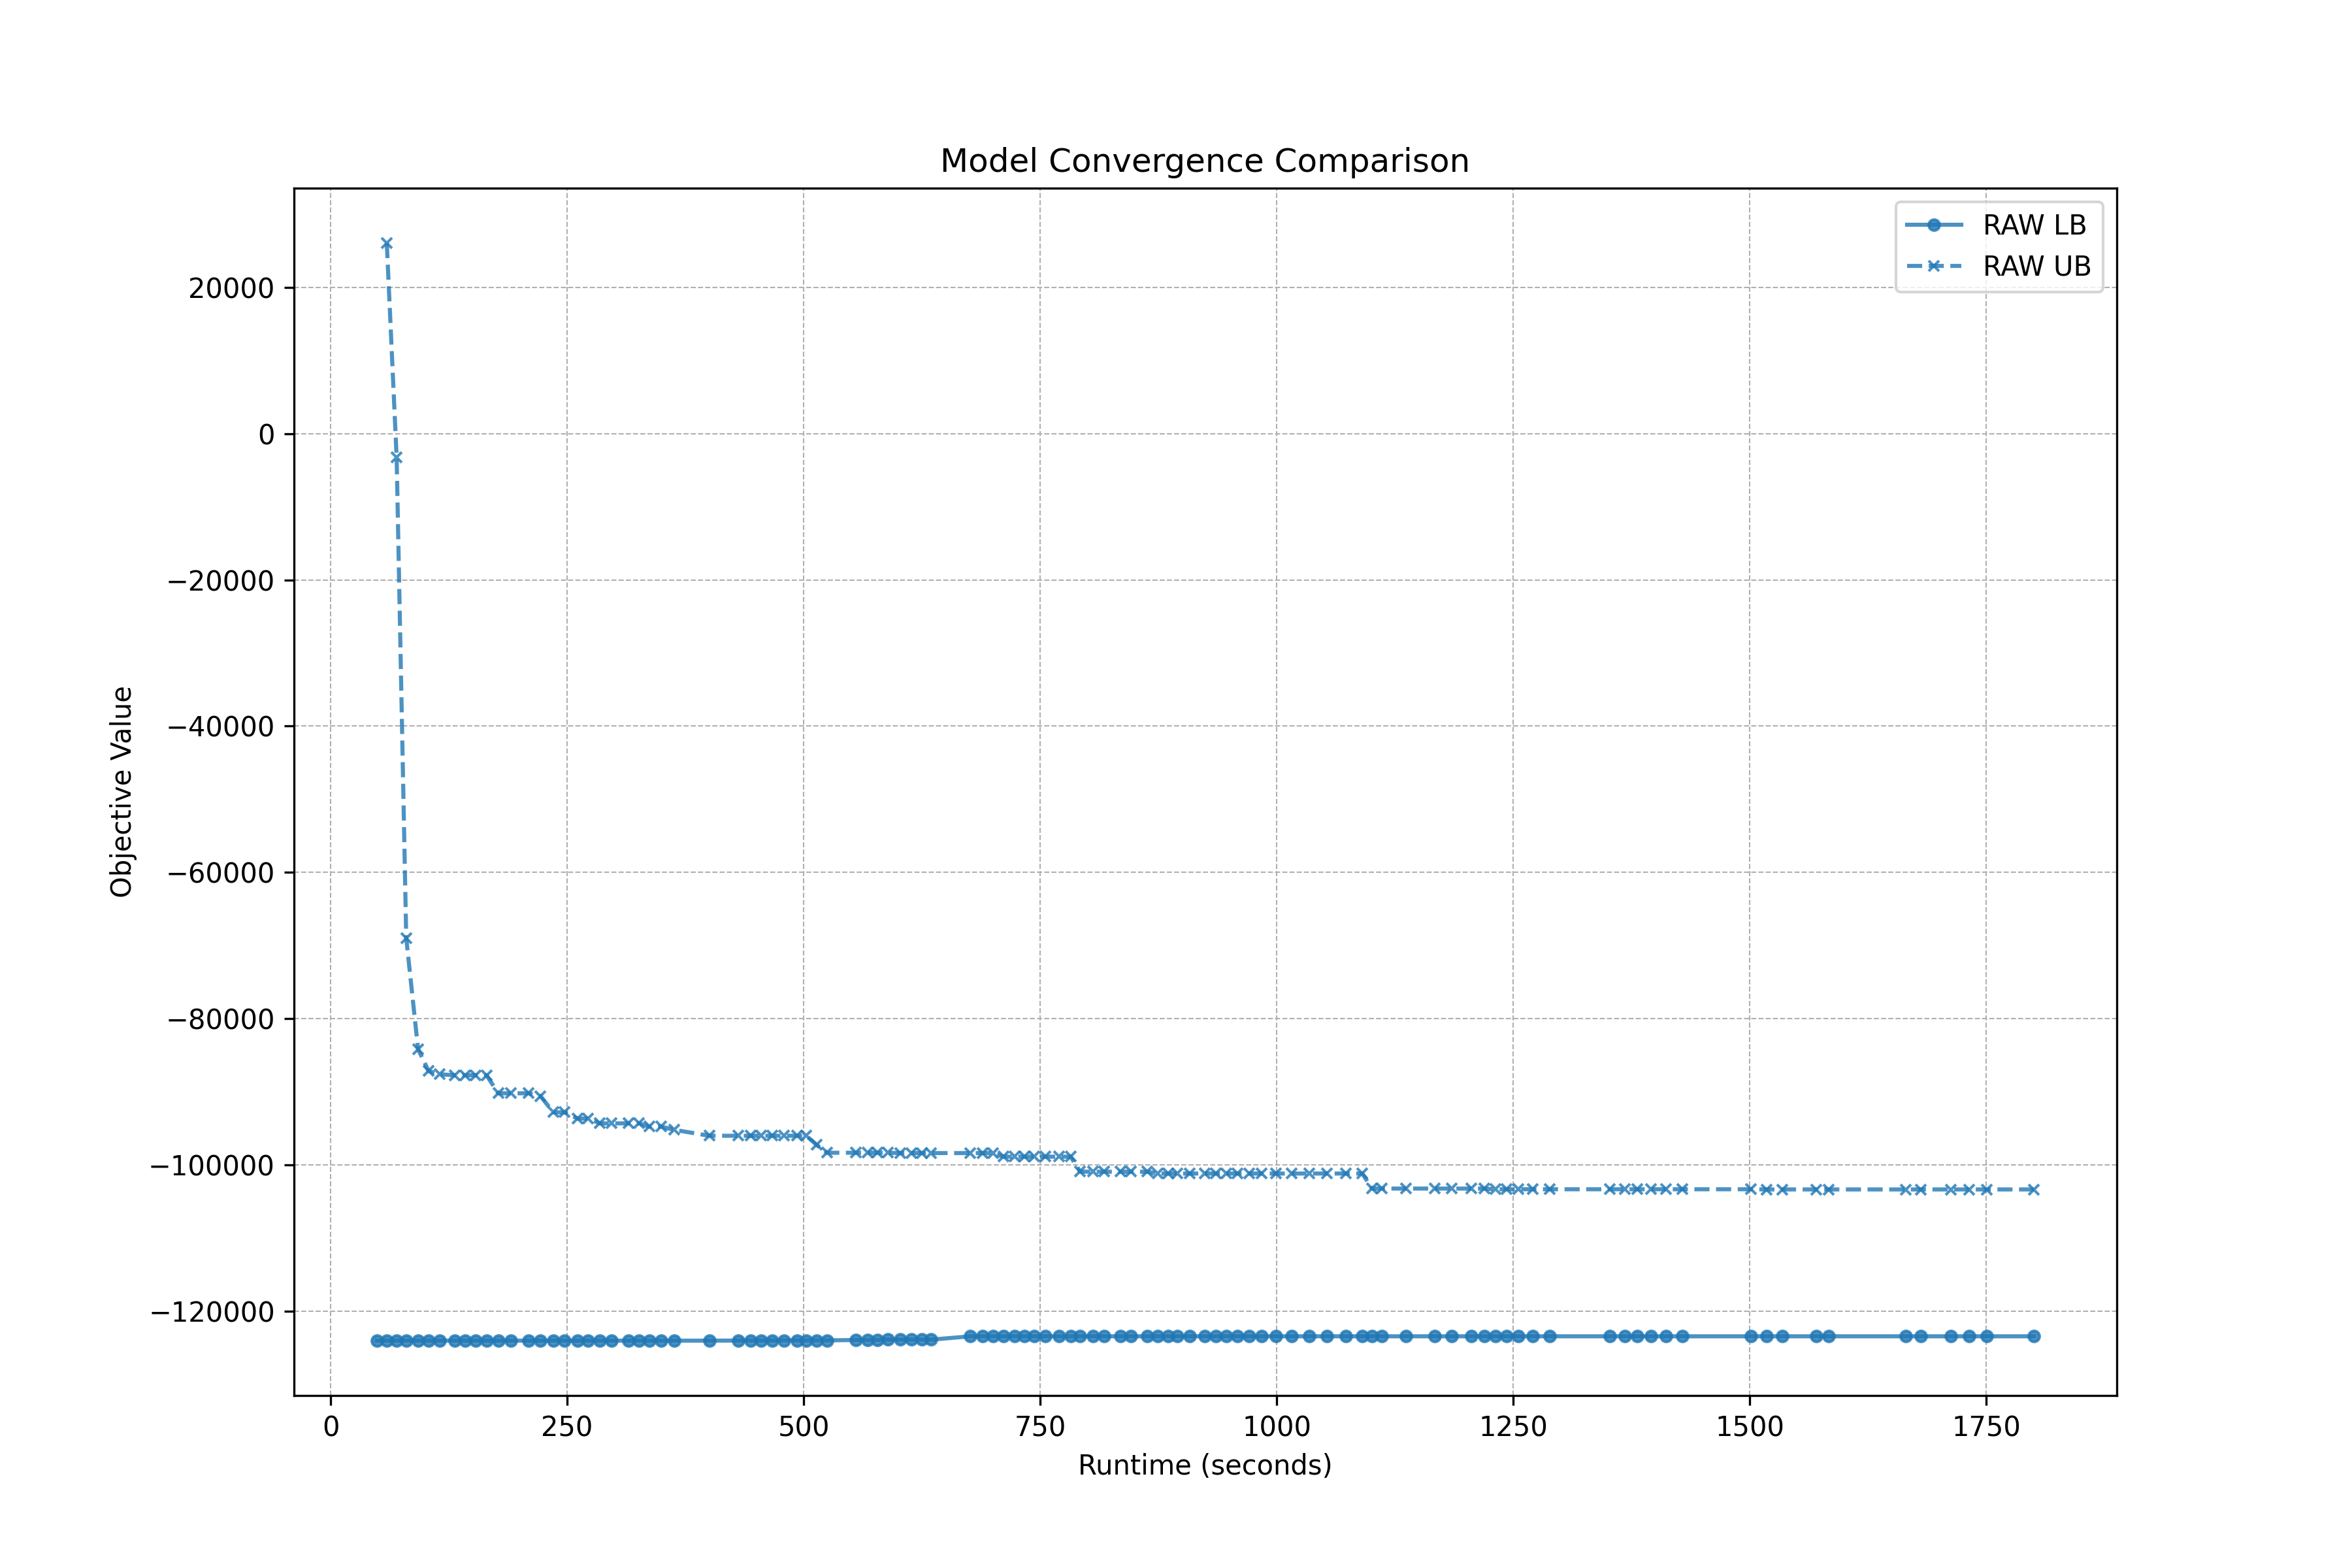
\includegraphics[width=0.8\textwidth]{figure/img/converge_f9_raw.png}
% %     \caption{Convergence Plot for F9, RAW}
% %     \label{fig:converge.f9.raw}
% % \end{figure}
% % \begin{figure}[h]
% %     \centering
% %     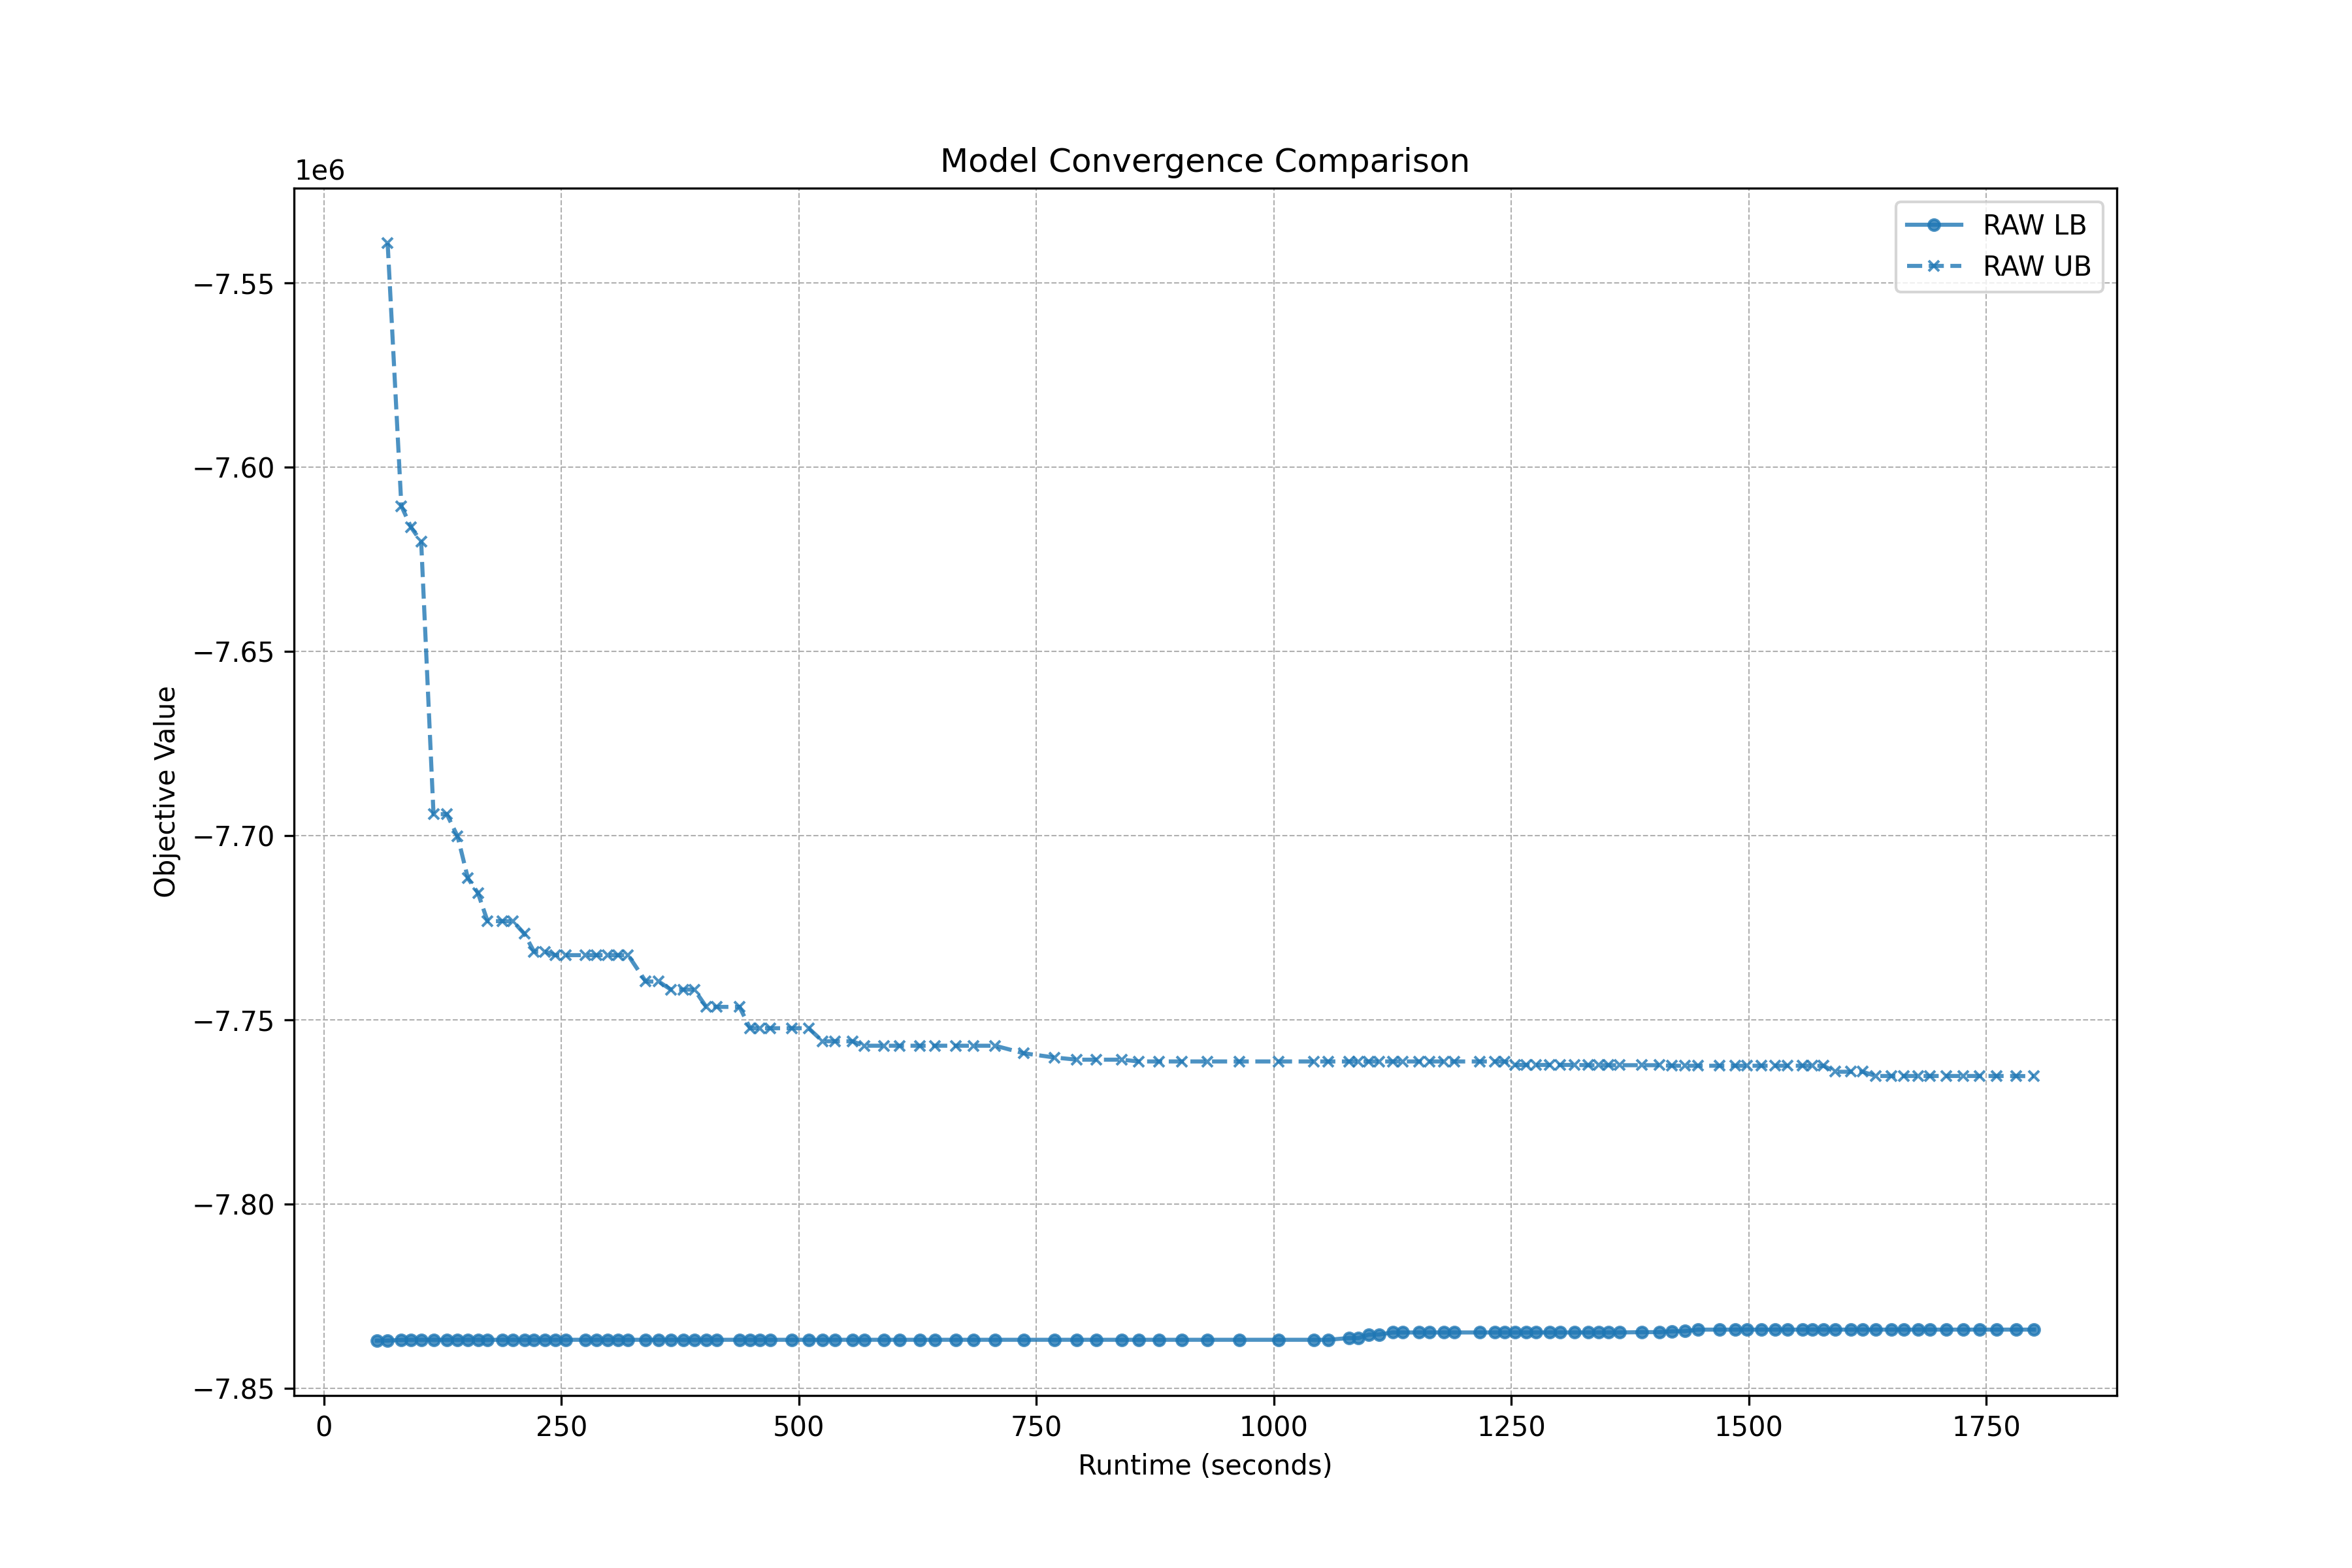
\includegraphics[width=0.8\textwidth]{figure/img/converge_b6_raw.png}
% %     \caption{Convergence Plot for B6, RAW}
% %     \label{fig:converge.b6.raw}
% % \end{figure}
% % \begin{figure}[h]
% %     \centering
% %     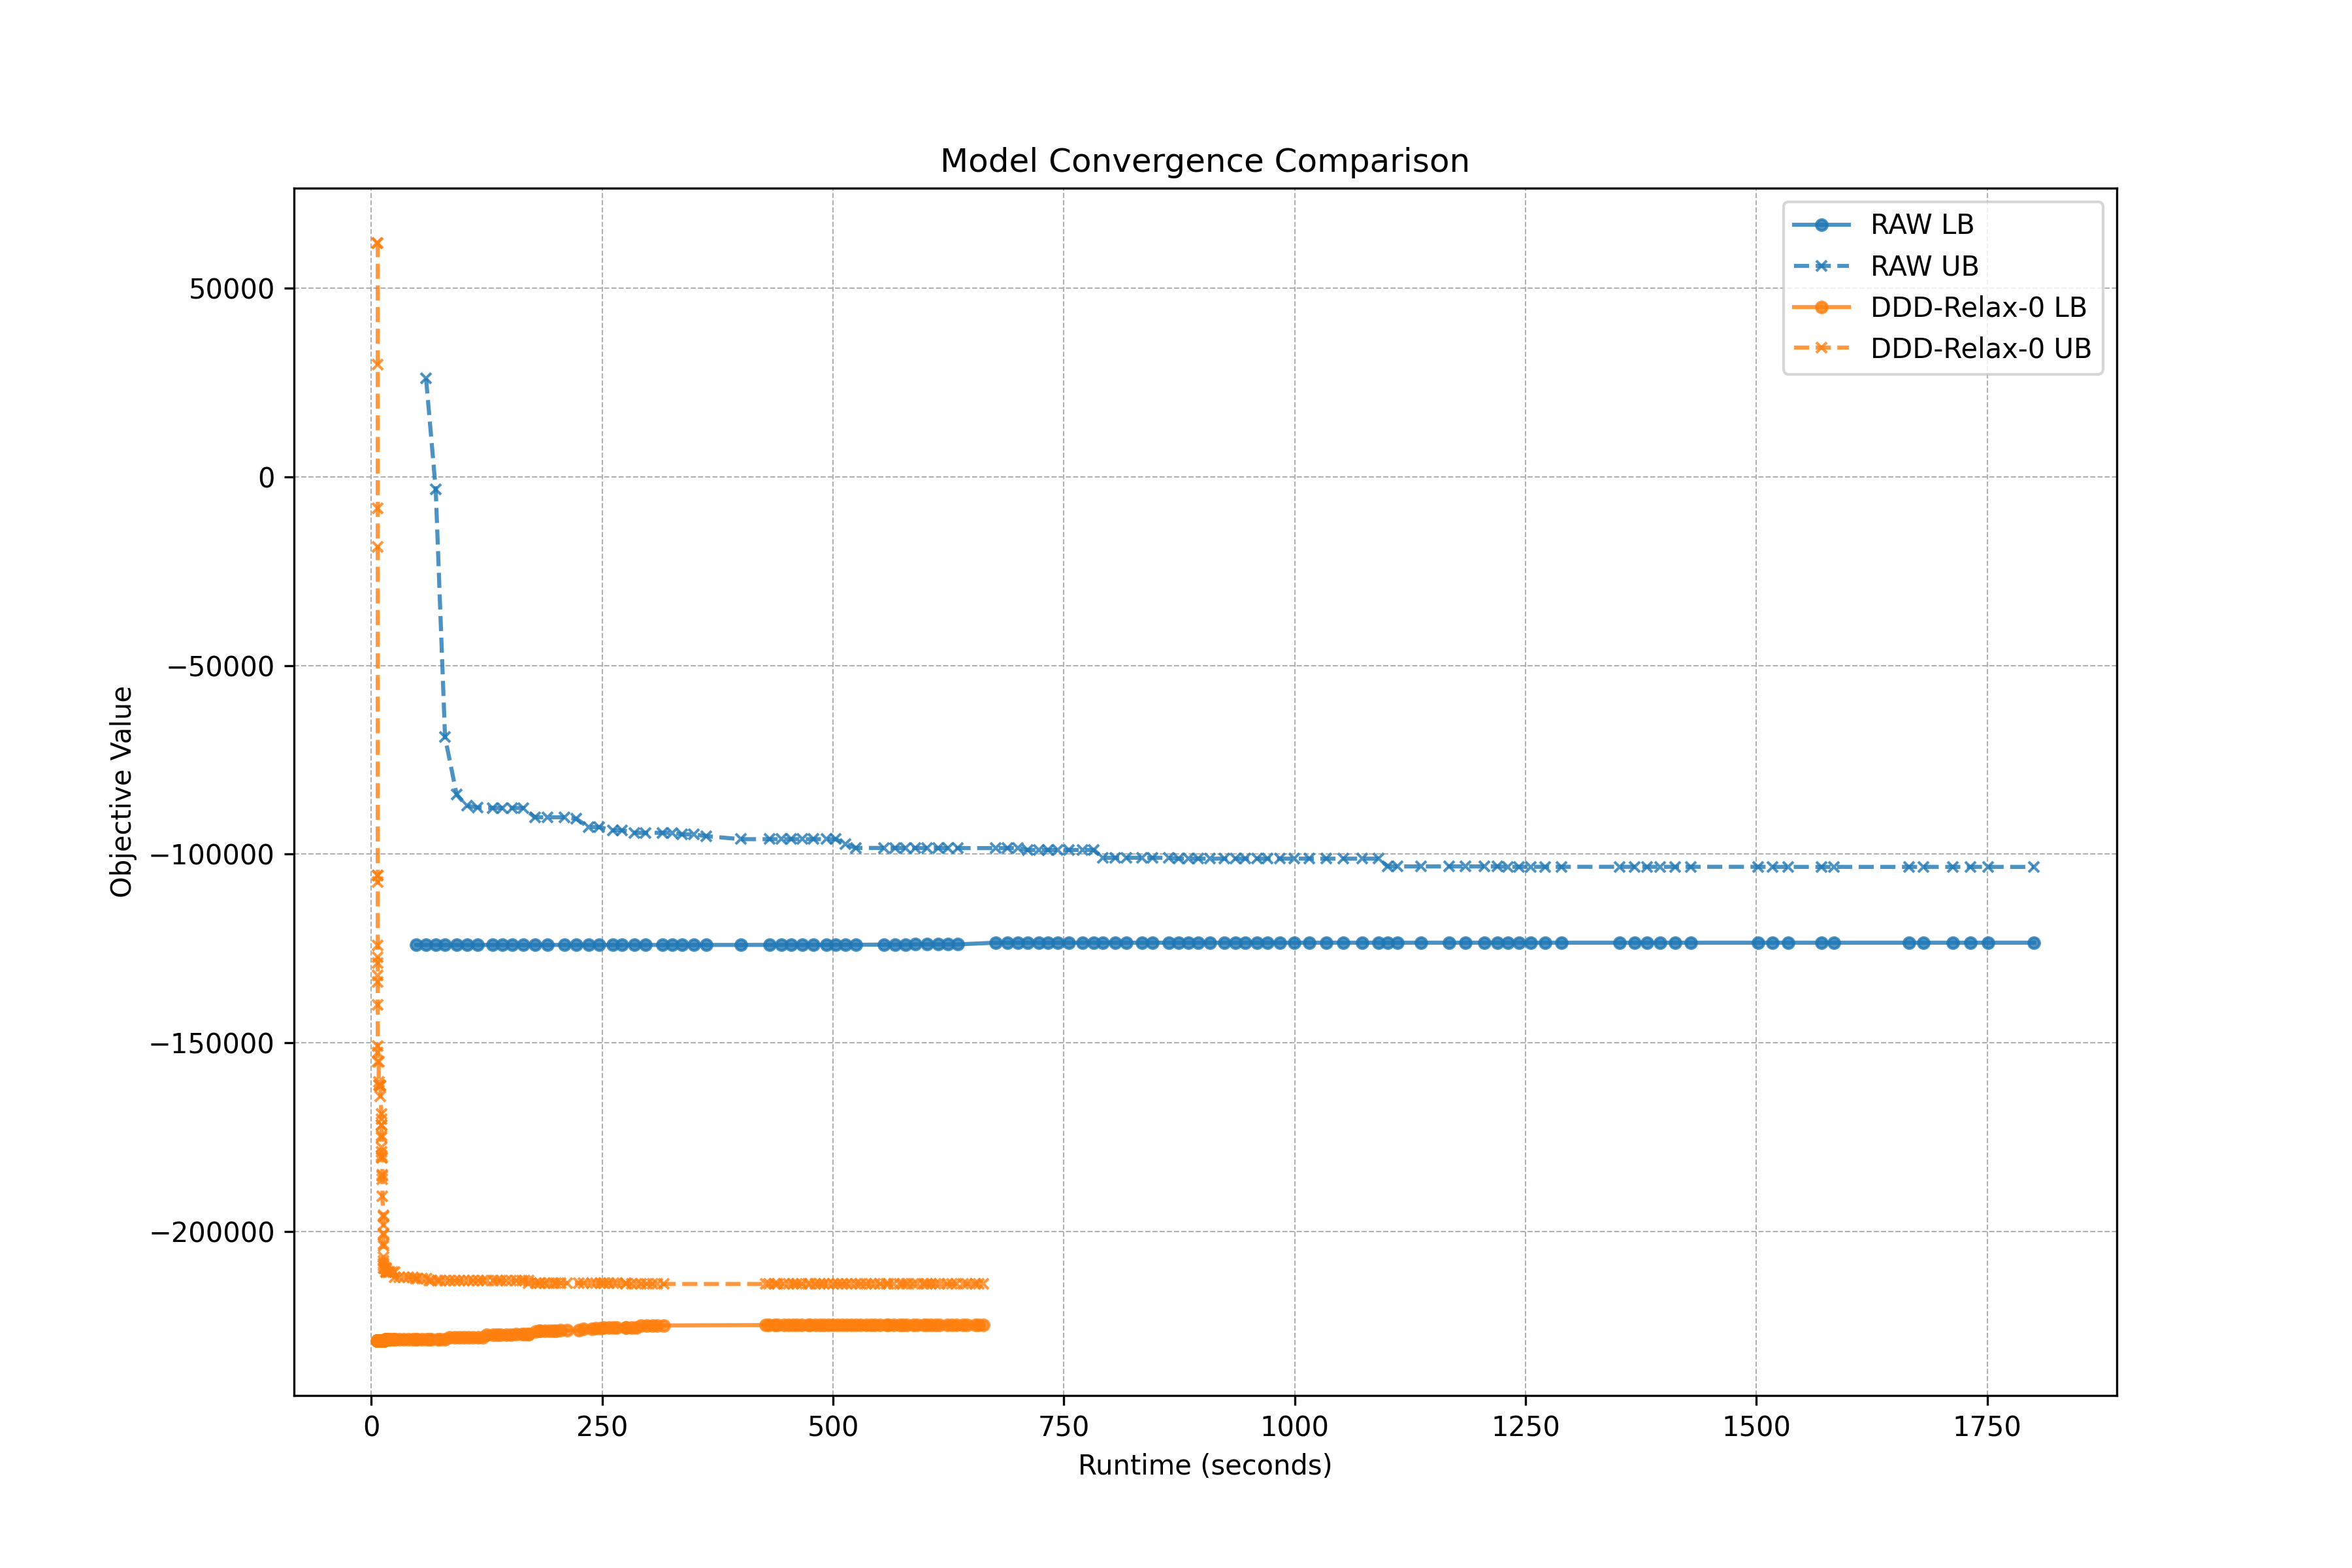
\includegraphics[width=0.8\textwidth]{figure/img/converge_f9_ddd_relax_0.png}
% %     \caption{Convergence Plot for F9, DDD-Relax, Method 0}
% %     \label{fig:converge.f9.ddd.r0}
% % \end{figure}
% % \begin{figure}[h]
% %     \centering
% %     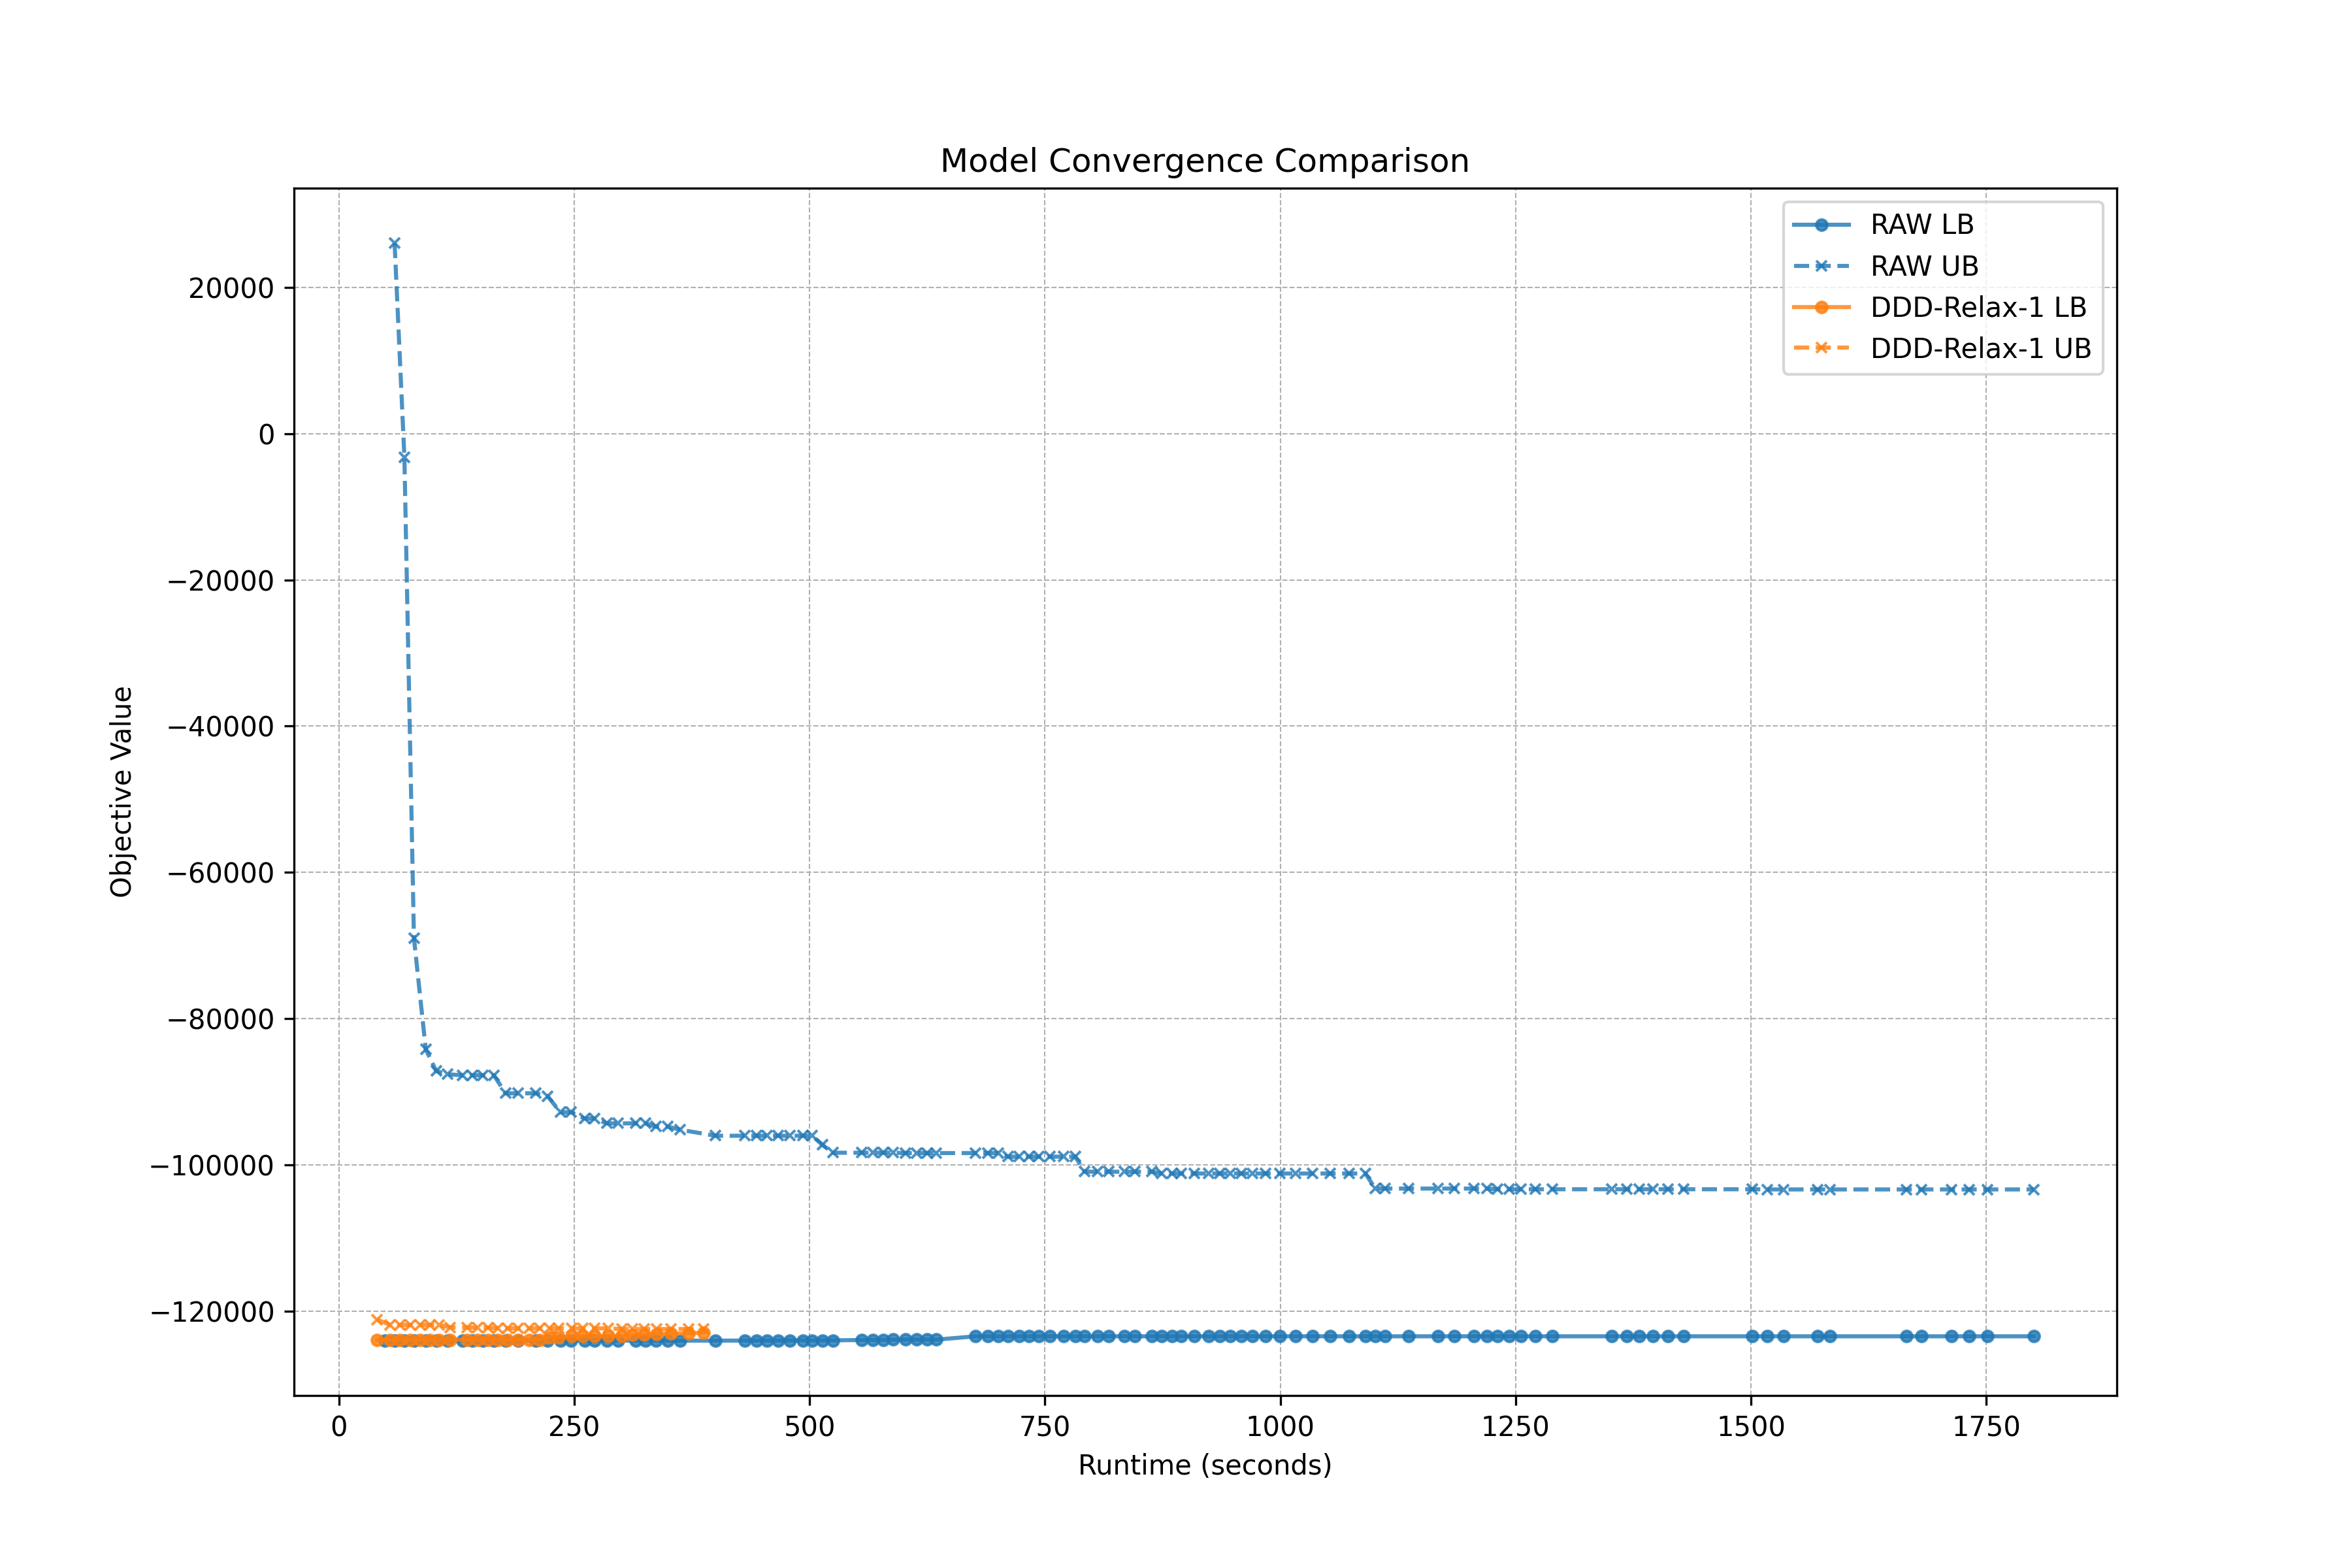
\includegraphics[width=0.8\textwidth]{figure/img/converge_f9_ddd_relax_1.png}
% %     \caption{Convergence Plot for F9, DDD-Relax, Method 1}
% %     \label{fig:converge.f9.ddd.r1}
% % \end{figure}
% % \begin{figure}[h]
% %     \centering
% %     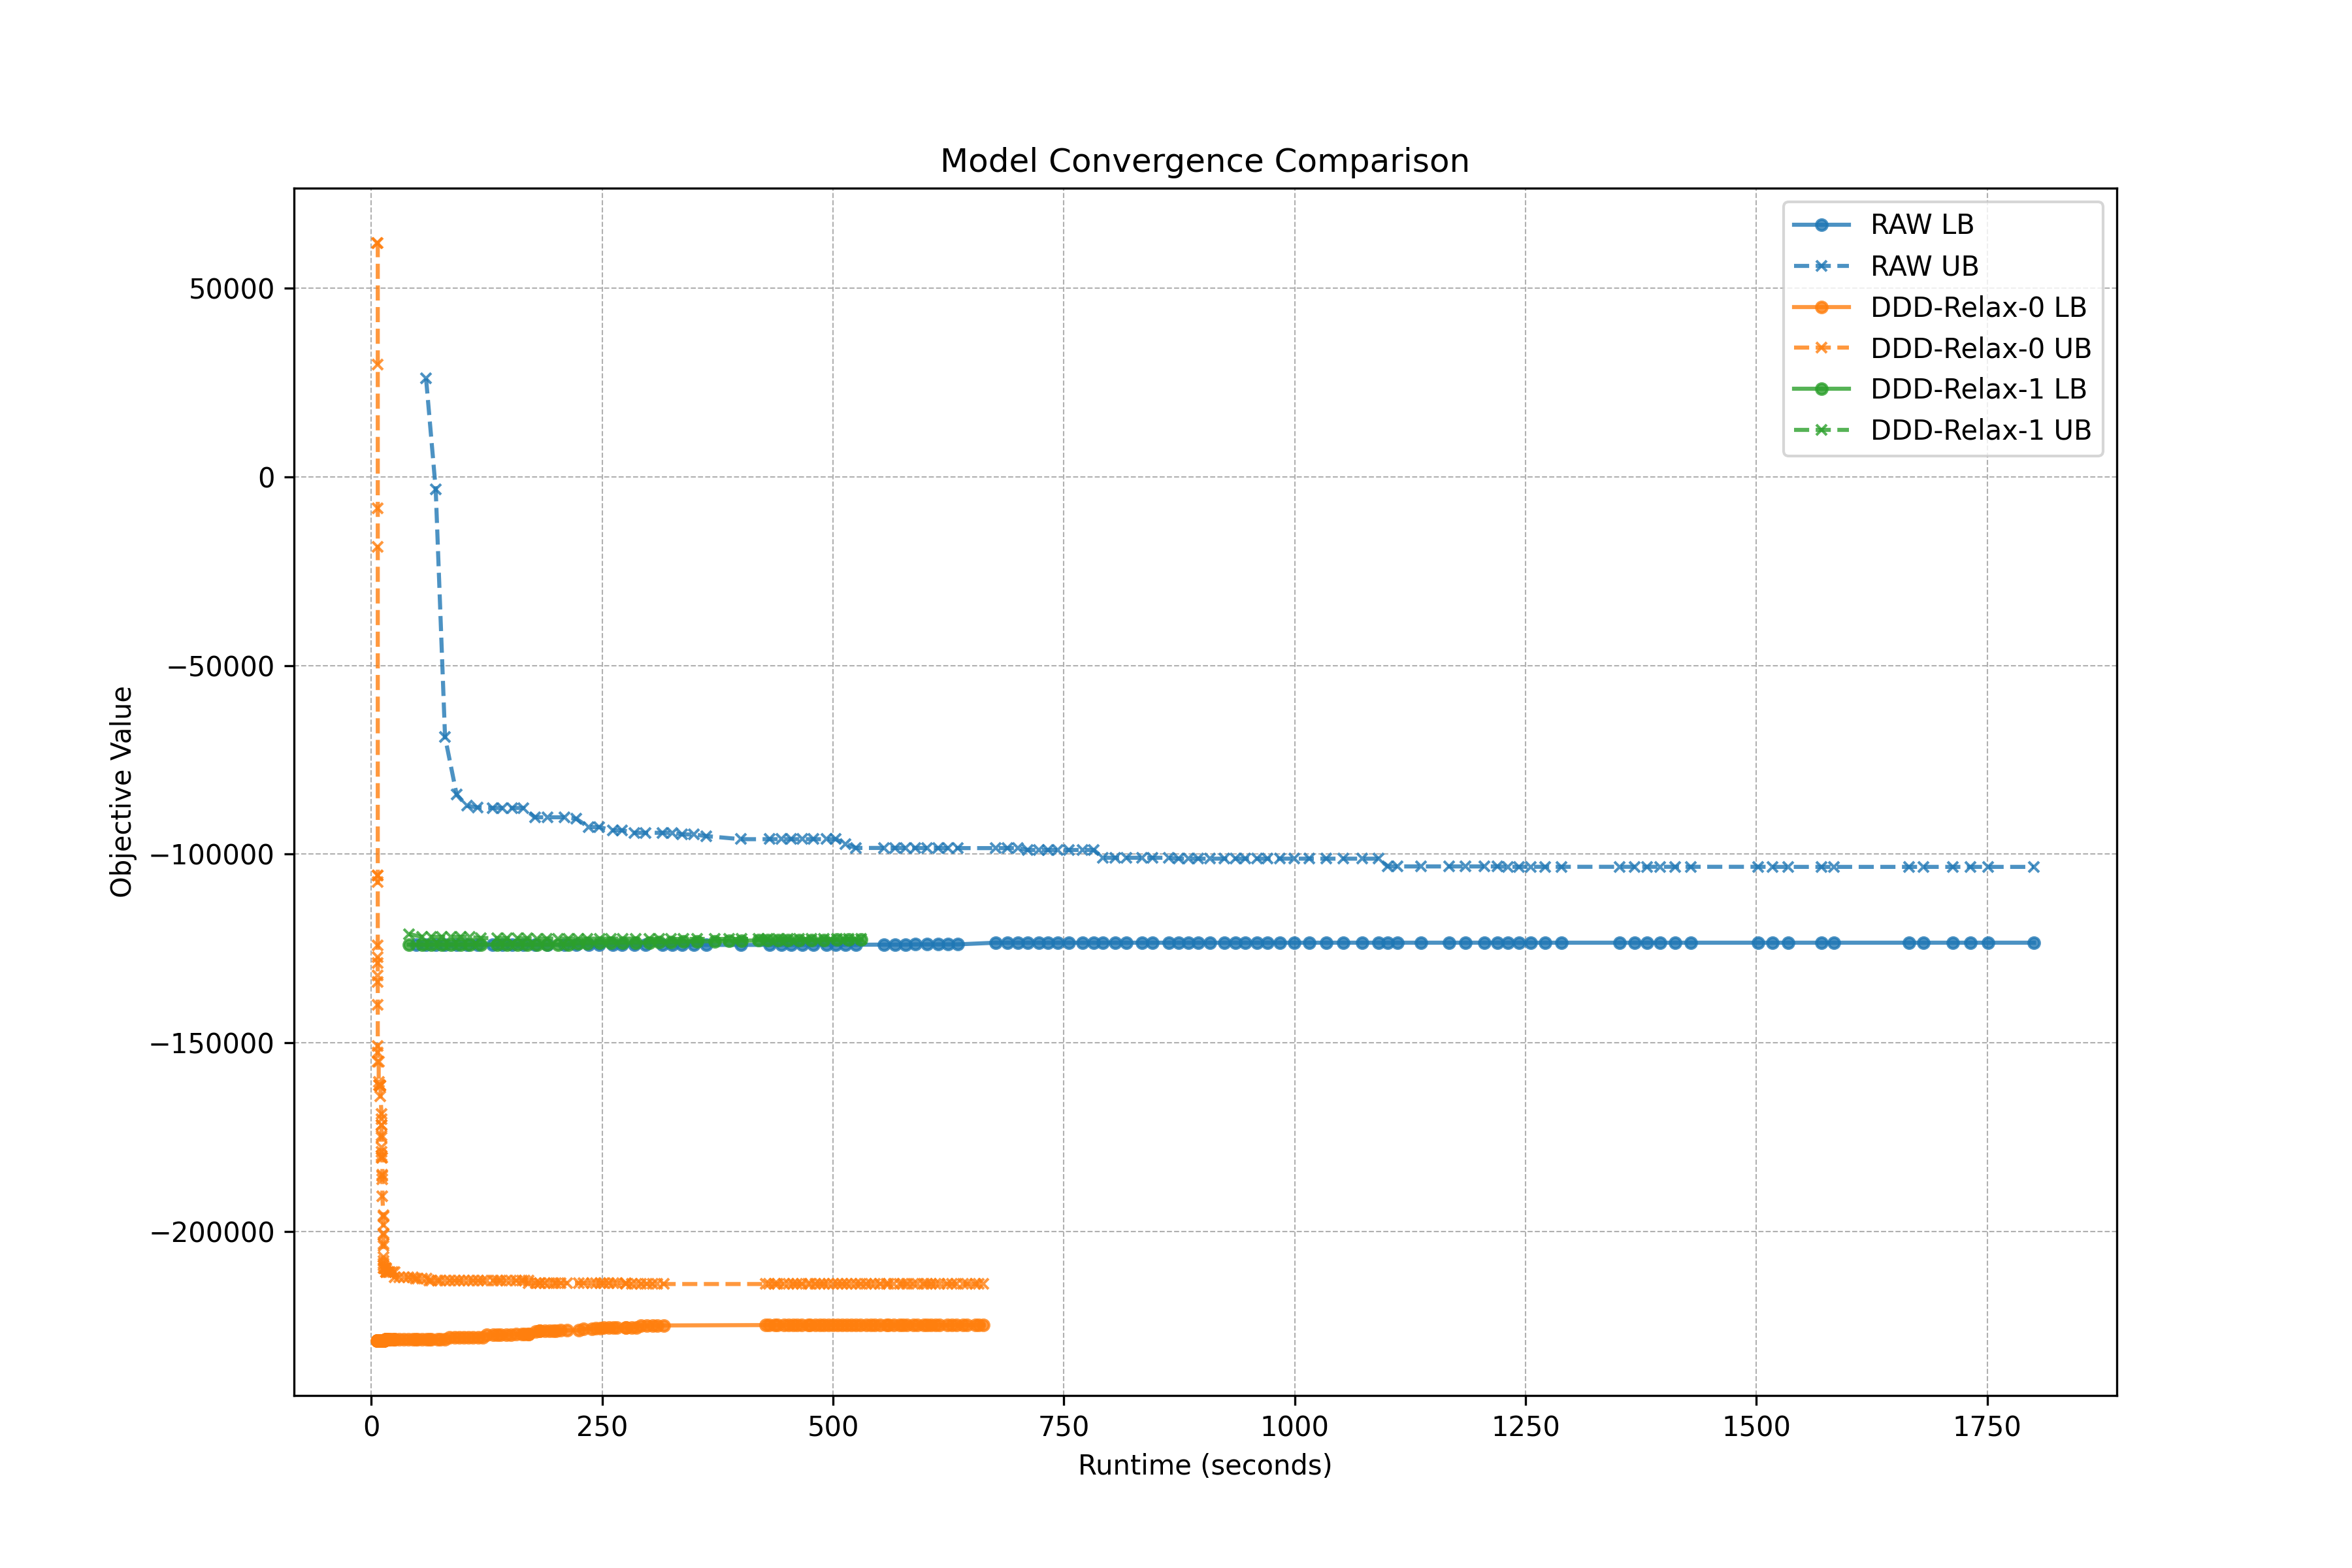
\includegraphics[width=0.8\textwidth]{figure/img/converge_f9_ddd_relax_01.png}
% %     \caption{Convergence Plot for F9, DDD-Relax, Method 0\&1}
% %     \label{fig:converge.f9.ddd.r0r1}
% % \end{figure}
% % \begin{figure}[h]
% %     \centering
% %     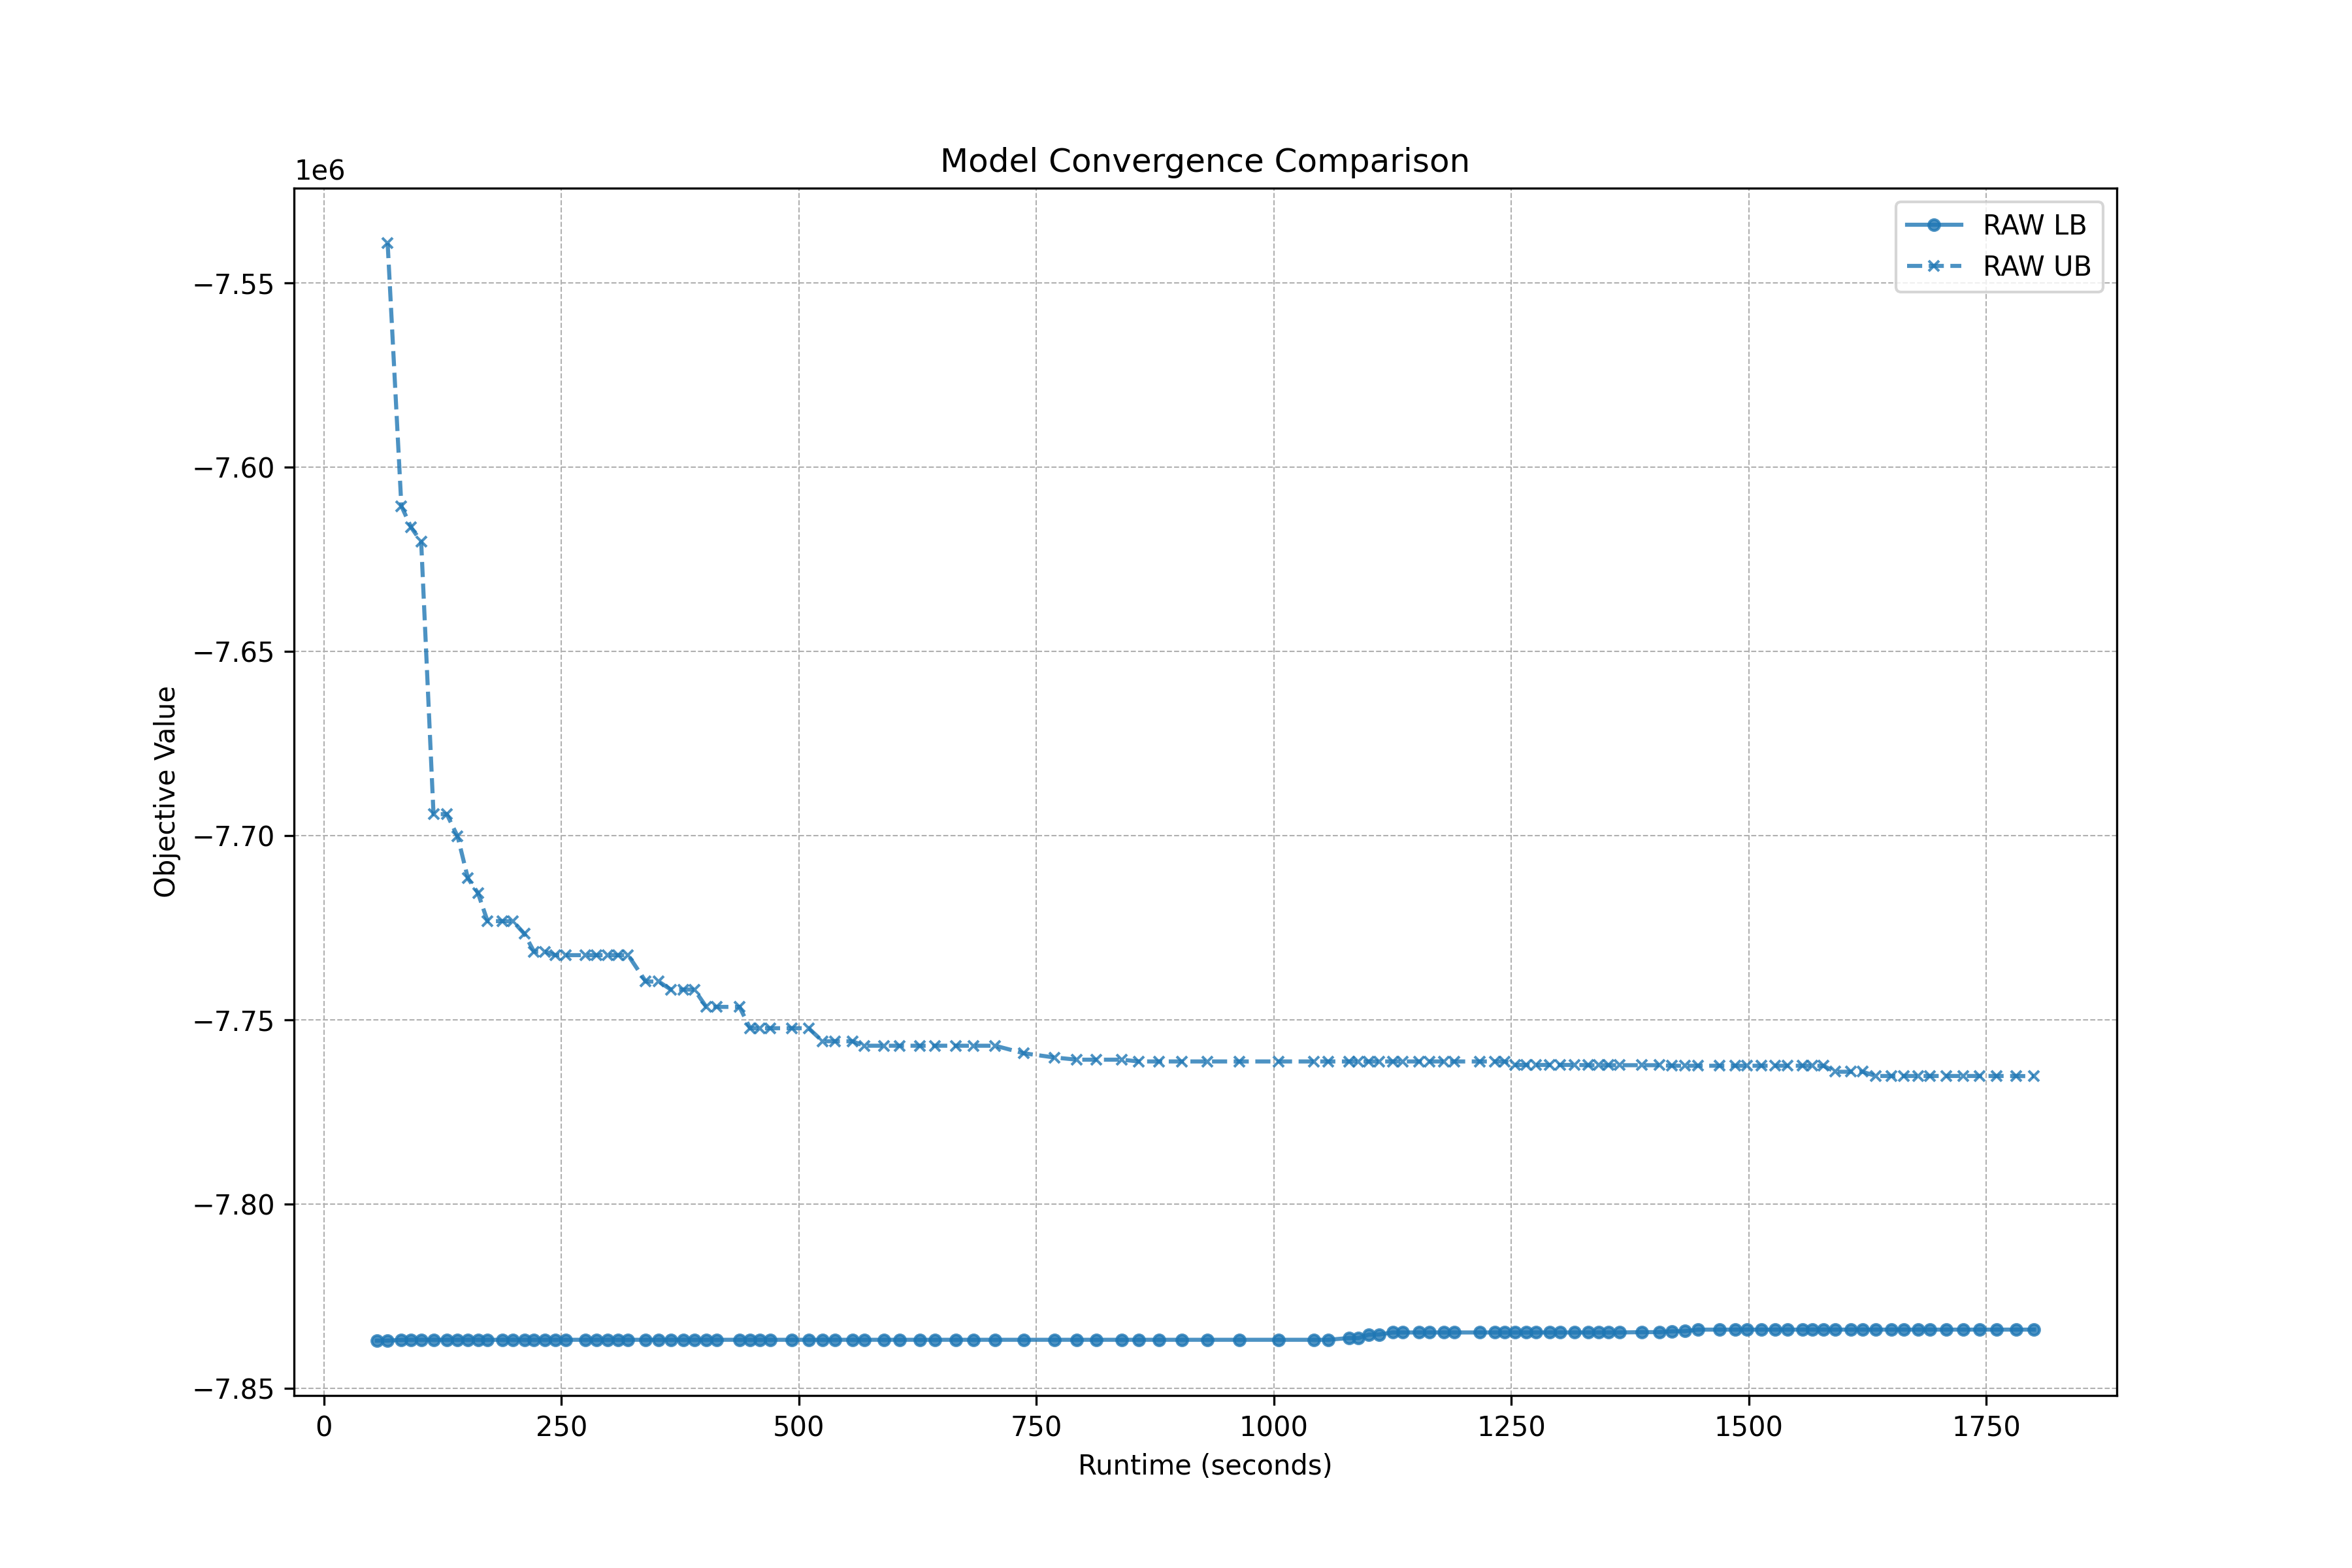
\includegraphics[width=0.8\textwidth]{figure/img/converge_b6_raw.png}
% %     \caption{Convergence Plot for B6, RAW}
% %     \label{fig:converge.b6.raw}
% % \end{figure}
% % \subsection{FDM and Upper Bound}
% % \subsection{Refine Strategy}

% \begin{figure}[ht]
%   \centering
%   \begin{subfigure}{0.48\textwidth}
%     \centering
%     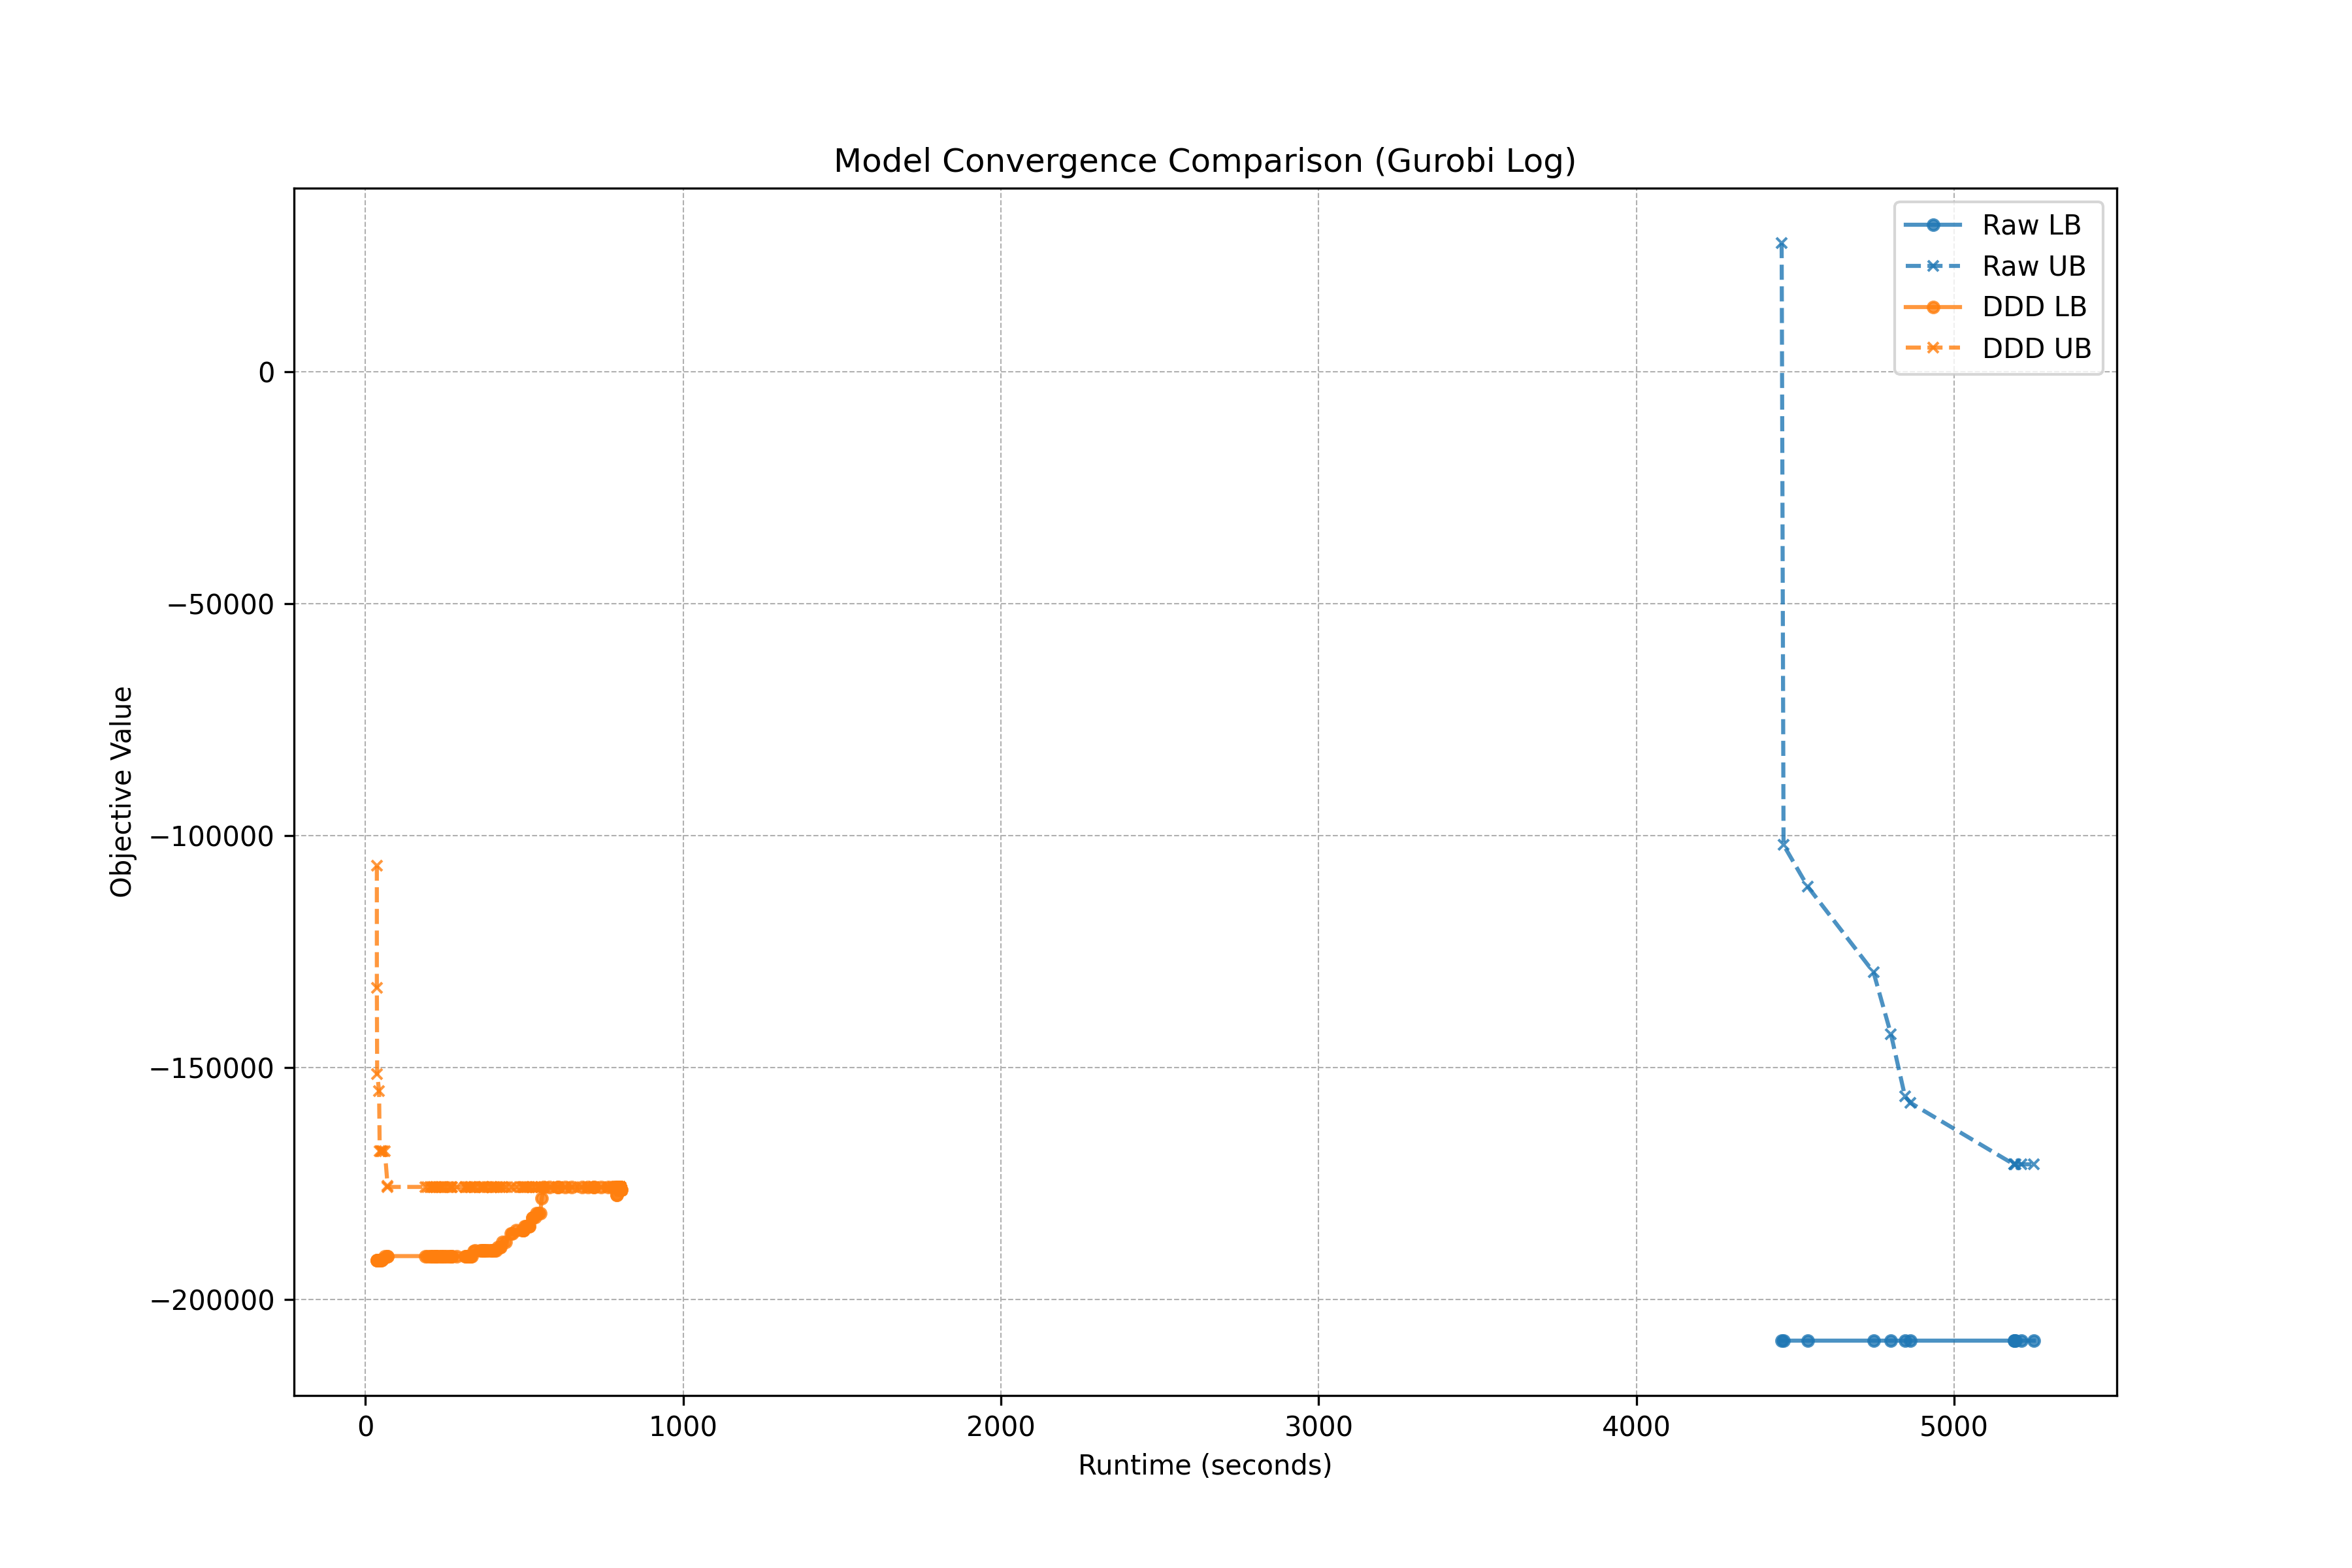
\includegraphics[width=\textwidth]{figure/img/converge_f9_nddd.png}
%     \caption{RAW vs DDD}
%     \label{fig:converge.f9.nddd}
%   \end{subfigure}
%   \hfill
%   \begin{subfigure}{0.48\textwidth}
%     \centering
%     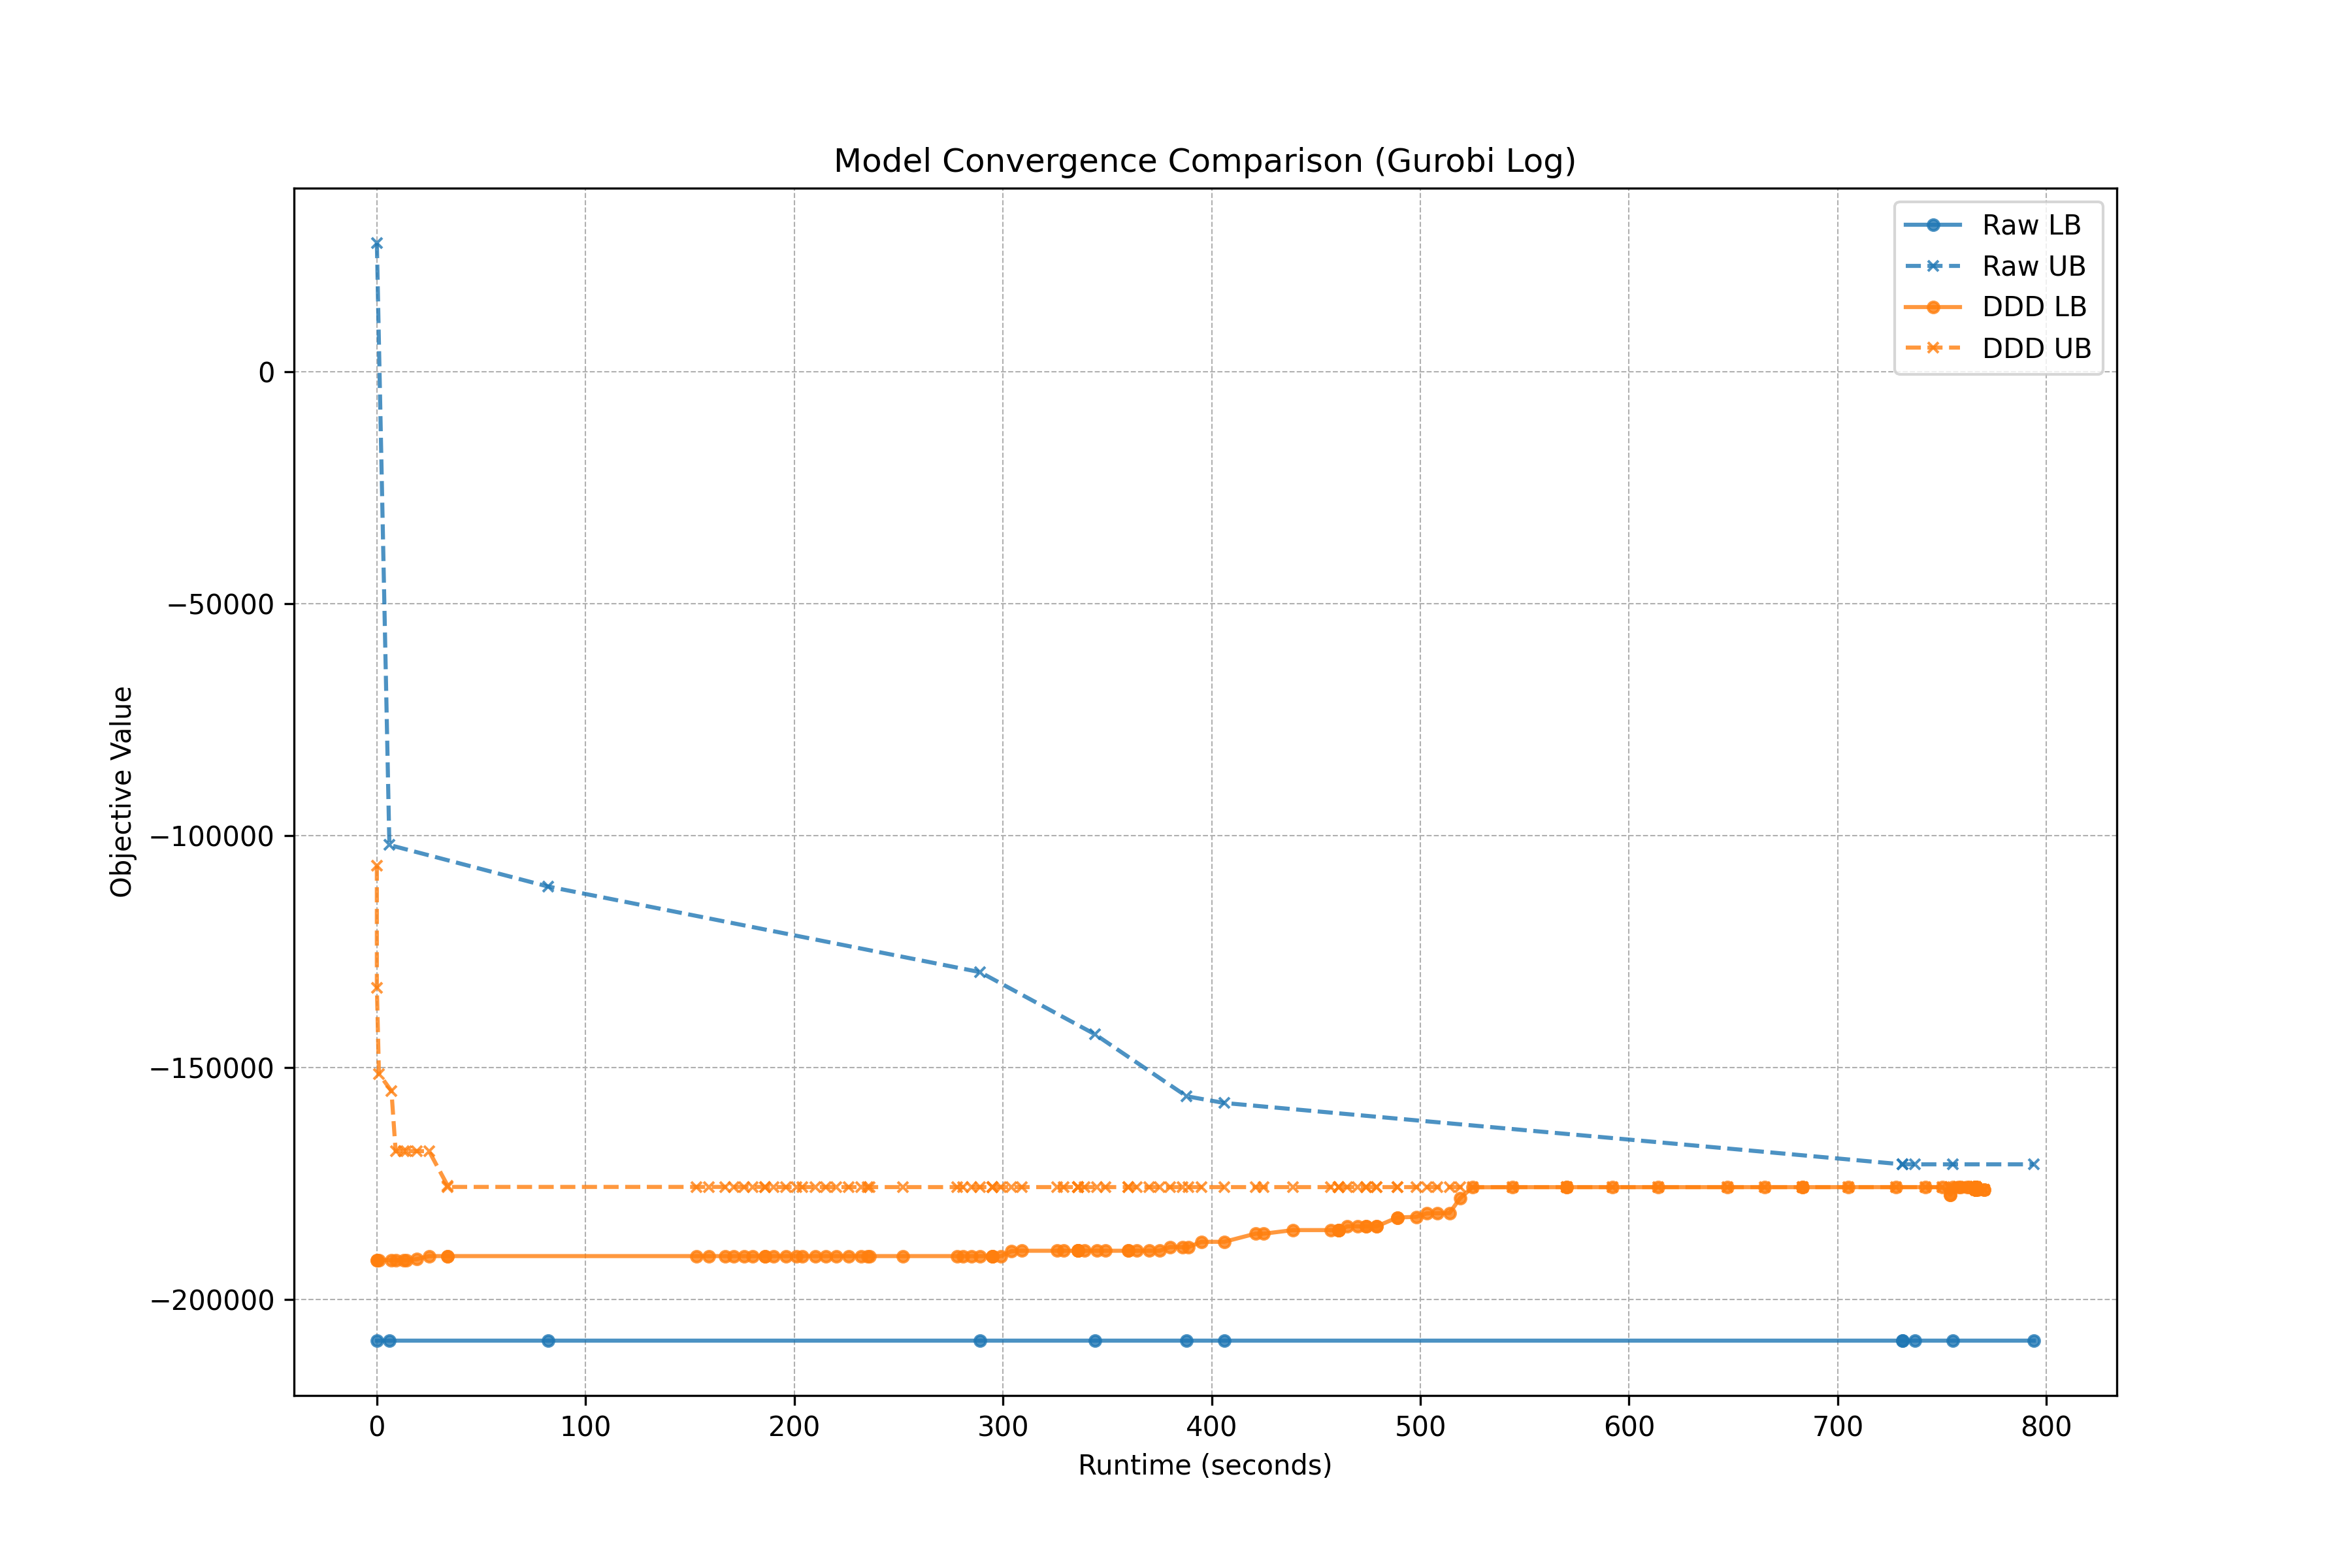
\includegraphics[width=\textwidth]{figure/img/converge_f9_nddd_aligned.png}
%     \caption{RAW vs DDD (Aligned)}
%     \label{fig:converge.f9.nddd.aligned}
%   \end{subfigure}
%   \caption{Convergence Plot for F9}
% \end{figure}

% Table \ref{tab:results_comparison} presents the computational solutions for the selected instance, comparing the performance of DDD against standard benchmarks. The proposed DDD framework (specifically the IDDD implementation) demonstrates superior performance. IDDD achieves the highest profit of \$176,403 with a remarkably tight global optimality gap of 0.24\%.This is achieved by effectively combining the strong lower bound from the relaxed model (IDDD-Relax, \$176,829) and the high-quality integer solution from the Vantage algorithm (IDDD-UB). In comparison, the direct implementation using the commercial solver Gurobi struggles to converge, yielding a significant 22.25\% gap and a lower profit (\$170,883) even after 5 hours of computation on a high-memory machine. The Multi-Phase decomposition method, while reporting a 0.00\% gap, converged to a significantly inferior local optimum (\$64,367), verifying that it fails to effectively explore the full search space. Thus, DDD provides the best computational efficiency (0.78 hours), and proof of optimality. 

% \begin{table}
% \caption{Comparison to Benchmarks\label{tab:results_comparison}}
% \centering
% \begin{tabular}{l c c c c}
% \toprule
% \textbf{Method} & \textbf{\% Gap} & \textbf{Profit (\$)} & \textbf{CPU (hr)} & \textbf{Status} \\
% \midrule
% \multirow{2}{*}{Gurobi Directly}
% & N/A & N/A & 0.67 & TL \\
% & 22.25 & 170,883.04 & 5.00 & SU \\
% [0.5em]
% \multirow{2}{*}{DDD} & N/A & N/A & 0.67 & TL \\
% & N/A & N/A & 5.00 & TL \\
% [0.5em]
% \multirow{2}{*}{Multi-Phase}
% & 17.3 & 64,336.39 & 0.67 & SU\\
% & 0.00 & 64,367.08 & 5.00 & C-SU\\
% [0.5em]
% \multirow{1}{*}{IDDD-Relax} & 0.00 & 176,829.19 & 0.11 & C-RE \\
% \multirow{1}{*}{IDDD-UB{\tiny (VANTAGE)}} & 0.00 & 176,403.40 & 0.67 & C-SU \\
% \multirow{1}{*}{IDDD} & 0.24 & 176,403.40 & 0.78 & C \\
% \bottomrule
% \end{tabular}

% {\tiny
% TL: Too long to find a solution;
% OOM: Out of memory error;
% SU: Suboptimal;
% RE: Relaxed;
% C: Converged.
% }
% \end{table}

% \begin{table}[htbp]
% \caption{Detailed Results for Solution (IDDD Case)}
% \centering
% \scriptsize
% \setlength{\tabcolsep}{2pt}
% \begin{tabular}{llrrrrrrrrr}
% \toprule
% Airline & Method & Type & Seg & Flt & Pax & Seat & Cost & Rev & PPF & LF \\
% \midrule
% \multirow{10}{*}{F9} 
% & \multirow{5}{*}{\shortstack[l]{RAW\\Obj: 175,519.34\\Gap: 19.02\%}}
% & H2H & 122 & 172 & 25,537.23 & 36,192 & 2,211,714.09 & 2,974,400.73 & 148.47 & 0.71 \\
% & & H2S & 52 & 86 & 4,920.27 & 17,112 & 1,307,002.48 & 578,732.87 & 57.21 & 0.29 \\
% & & S2H & 81 & 86 & 10,093.86 & 17,112 & 1,098,979.91 & 1,292,753.26 & 117.37 & 0.59 \\
% & & S2S & 4 & 4 & 0.00 & 768 & 52,671.04 & 0.00 & 0.00 & 0.00 \\
% & & \textbf{Total} & \textbf{259} & \textbf{348} & \textbf{40,551.36} & \textbf{71,184} & \textbf{4,670,367.52} & \textbf{4,845,886.86} & \textbf{116.53} & \textbf{0.57} \\
% \cmidrule{2-11}
% & \multirow{5}{*}{\shortstack[l]{IDDD\\Obj: 176,403.40\\Gap: 0.24\%}} 
% & H2H & 122 & 172 & 25,492.82 & 36,192 & 2,211,714.09 & 2,970,664.43 & 148.21 & 0.70 \\
% & & H2S & 52 & 86 & 4,959.33 & 17,112 & 1,307,002.48 & 584,333.71 & 57.67 & 0.29 \\
% & & S2H & 81 & 86 & 10,093.84 & 17,112 & 1,098,979.91 & 1,291,769.90 & 117.37 & 0.59 \\
% & & S2S & 4 & 4 & 0.00 & 768 & 52,671.04 & 0.00 & 0.00 & 0.00 \\
% & & \textbf{Total} & \textbf{259} & \textbf{348} & \textbf{40,545.99} & \textbf{71,184} & \textbf{4,670,367.52} & \textbf{4,846,768.05} & \textbf{116.51} & \textbf{0.57} \\
% \bottomrule
% \end{tabular}

% {\tiny
% Seg: Segment count;
% Flt: Flight count;
% Pax: Passenger count;
% PPF: Passenger per Flight;
% LF: Load Factor.
% }
% \end{table}

\TBD
